
%% bare_conf.tex
%% V1.3
%% 2007/01/11
%% by Michael Shell
%% See:
%% http://www.michaelshell.org/
%% for current contact information.
%%
%% This is a skeleton file demonstrating the use of IEEEtran.cls
%% (requires IEEEtran.cls version 1.7 or later) with an IEEE conference paper.
%%
%% Support sites:
%% http://www.michaelshell.org/tex/ieeetran/
%% http://www.ctan.org/tex-archive/macros/latex/contrib/IEEEtran/
%% and
%% http://www.ieee.org/

%%*************************************************************************
%% Legal Notice:
%% This code is offered as-is without any warranty either expressed or
%% implied; without even the implied warranty of MERCHANTABILITY or
%% FITNESS FOR A PARTICULAR PURPOSE! 
%% User assumes all risk.
%% In no event shall IEEE or any contributor to this code be liable for
%% any damages or losses, including, but not limited to, incidental,
%% consequential, or any other damages, resulting from the use or misuse
%% of any information contained here.
%%
%% All comments are the opinions of their respective authors and are not
%% necessarily endorsed by the IEEE.
%%
%% This work is distributed under the LaTeX Project Public License (LPPL)
%% ( http://www.latex-project.org/ ) version 1.3, and may be freely used,
%% distributed and modified. A copy of the LPPL, version 1.3, is included
%% in the base LaTeX documentation of all distributions of LaTeX released
%% 2003/12/01 or later.
%% Retain all contribution notices and credits.
%% ** Modified files should be clearly indicated as such, including  **
%% ** renaming them and changing author support contact information. **
%%
%% File list of work: IEEEtran.cls, IEEEtran_HOWTO.pdf, bare_adv.tex,
%%                    bare_conf.tex, bare_jrnl.tex, bare_jrnl_compsoc.tex
%%*************************************************************************

% *** Authors should verify (and, if needed, correct) their LaTeX system  ***
% *** with the testflow diagnostic prior to trusting their LaTeX platform ***
% *** with production work. IEEE's font choices can trigger bugs that do  ***
% *** not appear when using other class files.                            ***
% The testflow support page is at:
% http://www.michaelshell.org/tex/testflow/



% Note that the a4paper option is mainly intended so that authors in
% countries using A4 can easily print to A4 and see how their papers will
% look in print - the typesetting of the document will not typically be
% affected with changes in paper size (but the bottom and side margins will).
% Use the testflow package mentioned above to verify correct handling of
% both paper sizes by the user's LaTeX system.
%
% Also note that the "draftcls" or "draftclsnofoot", not "draft", option
% should be used if it is desired that the figures are to be displayed in
% draft mode.
%
% \documentclass[10pt, conference, letterpaper]{IEEEtran}
% \usepackage{amssymb}
% \usepackage{amstext}
% \usepackage{amsmath}
% %\usepackage{commonTemplates/algorithm}
% %\usepackage{commonTemplates/algorithmic}
% \usepackage{commonTemplates/subfigure}
% \usepackage{commonTemplates/graphicx}
% \usepackage{commonTemplates/graphics}
% \usepackage{commonTemplates/multirow}
% \usepackage[]{algorithm2e}
% \usepackage{color}
% %\usepackage{vmargin}
% %\usepackage[letter]{geometry}
% \special{papersize=8.5in,11in}
% \newtheorem{theorem}{Theorem}
% \newtheorem{acknowledgement}[theorem]{Acknowledgement}
% %\newtheorem{algorithm}[theorem]{Algorithm}
% \newtheorem{axiom}[theorem]{Axiom}
% \newtheorem{case}[theorem]{Case}
% \newtheorem{claim}[theorem]{Claim}
% \newtheorem{conclusion}[theorem]{Conclusion}
% \newtheorem{condition}[theorem]{Condition}
% \newtheorem{conjecture}[theorem]{Conjecture}
% \newtheorem{corollary}[theorem]{Corollary}
% \newtheorem{criterion}[theorem]{Criterion}
% \newtheorem{definition}[theorem]{Definition}
% \newtheorem{example}[theorem]{Example}
% \newtheorem{exercise}[theorem]{Exercise}
% \newtheorem{lemma}[theorem]{Lemma}
% \newtheorem{notation}[theorem]{Notation}
% \newtheorem{problem}[theorem]{Problem}
% \newtheorem{proposition}[theorem]{Proposition}
% \newtheorem{remark}[theorem]{Remark}
% \newtheorem{solution}[theorem]{Solution}
% \newtheorem{summary}[theorem]{Summary}
% \newcommand{\todo}[1]{\textcolor{red}{\textbf{{NILOY: #1}}}}

%
%\ifCLASSINFOpdf
  % \usepackage[pdftex]{graphicx}
  % declare the path(s) where your graphic files are
  % \graphicspath{{../pdf/}{../jpeg/}}
  % and their extensions so you won't have to specify these with
  % every instance of \includegraphics
  % \DeclareGraphicsExtensions{.pdf,.jpeg,.png}
%\else
  % or other class option (dvipsone, dvipdf, if not using dvips). graphicx
  % will default to the driver specified in the system graphics.cfg if no
  % driver is specified.
  % \usepackage[dvips]{graphicx}
  % declare the path(s) where your graphic files are
  % \graphicspath{{../eps/}}
  % and their extensions so you won't have to specify these with
  % every instance of \includegraphics
  % \DeclareGraphicsExtensions{.eps}
%\fi
% graphicx was written by David Carlisle and Sebastian Rahtz. It is
% required if you want graphics, photos, etc. graphicx.sty is already
% installed on most LaTeX systems. The latest version and documentation can
% be obtained at: 
% http://www.ctan.org/tex-archive/macros/latex/required/graphics/
% Another good source of documentation is "Using Imported Graphics in
% LaTeX2e" by Keith Reckdahl which can be found as epslatex.ps or
% epslatex.pdf at: http://www.ctan.org/tex-archive/info/
%
% latex, and pdflatex in dvi mode, support graphics in encapsulated
% postscript (.eps) format. pdflatex in pdf mode supports graphics
% in .pdf, .jpeg, .png and .mps (metapost) formats. Users should ensure
% that all non-photo figures use a vector format (.eps, .pdf, .mps) and
% not a bitmapped formats (.jpeg, .png). IEEE frowns on bitmapped formats
% which can result in "jaggedy"/blurry rendering of lines and letters as
% well as large increases in file sizes.
%
% You can find documentation about the pdfTeX application at:
% http://www.tug.org/applications/pdftex





% *** MATH PACKAGES ***
%
%\usepackage[cmex10]{amsmath}
% A popular package from the American Mathematical Society that provides
% many useful and powerful commands for dealing with mathematics. If using
% it, be sure to load this package with the cmex10 option to ensure that
% only type 1 fonts will utilized at all point sizes. Without this option,
% it is possible that some math symbols, particularly those within
% footnotes, will be rendered in bitmap form which will result in a
% document that can not be IEEE Xplore compliant!
%
% Also, note that the amsmath package sets \interdisplaylinepenalty to 10000
% thus preventing page breaks from occurring within multiline equations. Use:
%\interdisplaylinepenalty=2500
% after loading amsmath to restore such page breaks as IEEEtran.cls normally
% does. amsmath.sty is already installed on most LaTeX systems. The latest
% version and documentation can be obtained at:
% http://www.ctan.org/tex-archive/macros/latex/required/amslatex/math/





% *** SPECIALIZED LIST PACKAGES ***
%
%\usepackage{algorithmic}
% algorithmic.sty was written by Peter Williams and Rogerio Brito.
% This package provides an algorithmic environment fo describing algorithms.
% You can use the algorithmic environment in-text or within a figure
% environment to provide for a floating algorithm. Do NOT use the algorithm
% floating environment provided by algorithm.sty (by the same authors) or
% algorithm2e.sty (by Christophe Fiorio) as IEEE does not use dedicated
% algorithm float types and packages that provide these will not provide
% correct IEEE style captions. The latest version and documentation of
% algorithmic.sty can be obtained at:
% http://www.ctan.org/tex-archive/macros/latex/contrib/algorithms/
% There is also a support site at:
% http://algorithms.berlios.de/index.html
% Also of interest may be the (relatively newer and more customizable)
% algorithmicx.sty package by Szasz Janos:
% http://www.ctan.org/tex-archive/macros/latex/contrib/algorithmicx/




% *** ALIGNMENT PACKAGES ***
%
%\usepackage{array}
% Frank Mittelbach's and David Carlisle's array.sty patches and improves
% the standard LaTeX2e array and tabular environments to provide better
% appearance and additional user controls. As the default LaTeX2e table
% generation code is lacking to the point of almost being broken with
% respect to the quality of the end results, all users are strongly
% advised to use an enhanced (at the very least that provided by array.sty)
% set of table tools. array.sty is already installed on most systems. The
% latest version and documentation can be obtained at:
% http://www.ctan.org/tex-archive/macros/latex/required/tools/


%\usepackage{mdwmath}
%\usepackage{mdwtab}
% Also highly recommended is Mark Wooding's extremely powerful MDW tools,
% especially mdwmath.sty and mdwtab.sty which are used to format equations
% and tables, respectively. The MDWtools set is already installed on most
% LaTeX systems. The lastest version and documentation is available at:
% http://www.ctan.org/tex-archive/macros/latex/contrib/mdwtools/


% IEEEtran contains the IEEEeqnarray family of commands that can be used to
% generate multiline equations as well as matrices, tables, etc., of high
% quality.


%\usepackage{eqparbox}
% Also of notable interest is Scott Pakin's eqparbox package for creating
% (automatically sized) equal width boxes - aka "natural width parboxes".
% Available at:
% http://www.ctan.org/tex-archive/macros/latex/contrib/eqparbox/





% *** SUBFIGURE PACKAGES ***
%\usepackage[tight,footnotesize]{subfigure}
% subfigure.sty was written by Steven Douglas Cochran. This package makes it
% easy to put subfigures in your figures. e.g., "Figure 1a and 1b". For IEEE
% work, it is a good idea to load it with the tight package option to reduce
% the amount of white space around the subfigures. subfigure.sty is already
% installed on most LaTeX systems. The latest version and documentation can
% be obtained at:
% http://www.ctan.org/tex-archive/obsolete/macros/latex/contrib/subfigure/
% subfigure.sty has been superceeded by subfig.sty.



%\usepackage[caption=false]{caption}
%\usepackage[font=footnotesize]{subfig}
% subfig.sty, also written by Steven Douglas Cochran, is the modern
% replacement for subfigure.sty. However, subfig.sty requires and
% automatically loads Axel Sommerfeldt's caption.sty which will override
% IEEEtran.cls handling of captions and this will result in nonIEEE style
% figure/table captions. To prevent this problem, be sure and preload
% caption.sty with its "caption=false" package option. This is will preserve
% IEEEtran.cls handing of captions. Version 1.3 (2005/06/28) and later 
% (recommended due to many improvements over 1.2) of subfig.sty supports
% the caption=false option directly:
%\usepackage[caption=false,font=footnotesize]{subfig}
%
% The latest version and documentation can be obtained at:
% http://www.ctan.org/tex-archive/macros/latex/contrib/subfig/
% The latest version and documentation of caption.sty can be obtained at:
% http://www.ctan.org/tex-archive/macros/latex/contrib/caption/




% *** FLOAT PACKAGES ***
%
%\usepackage{fixltx2e}
% fixltx2e, the successor to the earlier fix2col.sty, was written by
% Frank Mittelbach and David Carlisle. This package corrects a few problems
% in the LaTeX2e kernel, the most notable of which is that in current
% LaTeX2e releases, the ordering of single and double column floats is not
% guaranteed to be preserved. Thus, an unpatched LaTeX2e can allow a
% single column figure to be placed prior to an earlier double column
% figure. The latest version and documentation can be found at:
% http://www.ctan.org/tex-archive/macros/latex/base/



%\usepackage{stfloats}
% stfloats.sty was written by Sigitas Tolusis. This package gives LaTeX2e
% the ability to do double column floats at the bottom of the page as well
% as the top. (e.g., "\begin{figure*}[!b]" is not normally possible in
% LaTeX2e). It also provides a command:
%\fnbelowfloat
% to enable the placement of footnotes below bottom floats (the standard
% LaTeX2e kernel puts them above bottom floats). This is an invasive package
% which rewrites many portions of the LaTeX2e float routines. It may not work
% with other packages that modify the LaTeX2e float routines. The latest
% version and documentation can be obtained at:
% http://www.ctan.org/tex-archive/macros/latex/contrib/sttools/
% Documentation is contained in the stfloats.sty comments as well as in the
% presfull.pdf file. Do not use the stfloats baselinefloat ability as IEEE
% does not allow \baselineskip to stretch. Authors submitting work to the
% IEEE should note that IEEE rarely uses double column equations and
% that authors should try to avoid such use. Do not be tempted to use the
% cuted.sty or midfloat.sty packages (also by Sigitas Tolusis) as IEEE does
% not format its papers in such ways.





% *** PDF, URL AND HYPERLINK PACKAGES ***
%
%\usepackage{url}
% url.sty was written by Donald Arseneau. It provides better support for
% handling and breaking URLs. url.sty is already installed on most LaTeX
% systems. The latest version can be obtained at:
% http://www.ctan.org/tex-archive/macros/latex/contrib/misc/
% Read the url.sty source comments for usage information. Basically,
% \url{my_url_here}.





% *** Do not adjust lengths that control margins, column widths, etc. ***
% *** Do not use packages that alter fonts (such as pslatex).         ***
% There should be no need to do such things with IEEEtran.cls V1.6 and later.
% (Unless specifically asked to do so by the journal or conference you plan
% to submit to, of course. )


% correct bad hyphenation here
% \hyphenation{op-tical net-works semi-conduc-tor}
% 
% 
% \begin{document}
% %
% % paper title
% % can use linebreaks \\ within to get better formatting as desired
% \title{On the broadcast of segmented messages \\ in dynamic networks}


% author names and affiliations
% use a multiple column layout for up to three different
% affiliations


% \author{\IEEEauthorblockN{Michael Shell}
% \IEEEauthorblockA{School of Electrical and\\Computer Engineering\\
% Georgia Institute of Technology\\
% Atlanta, Georgia 30332--0250\\
% Email: http://www.michaelshell.org/contact.html}
% \and
% \IEEEauthorblockN{Homer Simpson}
% \IEEEauthorblockA{Twentieth Century Fox\\
% Springfield, USA\\
% Email: homer@thesimpsons.com}
% \and
% \IEEEauthorblockN{James Kirk\\ and Montgomery Scott}
% \IEEEauthorblockA{Starfleet Academy\\
% San Francisco, California 96678-2391\\
% Telephone: (800) 555--1212\\
% Fax: (888) 555--1212}}

% conference papers do not typically use \thanks and this command
% is locked out in conference mode. If really needed, such as for
% the acknowledgment of grants, issue a \IEEEoverridecommandlockouts
% after \documentclass

% for over three affiliations, or if they all won't fit within the width
% of the page, use this alternative format:
% 
% \author{\IEEEauthorblockN{Sandipan Sikdar\IEEEauthorrefmark{1},
% Marcin Bodych\IEEEauthorrefmark{2},
% Rajib Ranjan Maiti\IEEEauthorrefmark{3},
% Biswajit Paria\IEEEauthorrefmark{1}\\
% Niloy Ganguly\IEEEauthorrefmark{1},
% Tyll Krueger\IEEEauthorrefmark{2}
% Animesh Mukherjee\IEEEauthorrefmark{1}}
% \IEEEauthorblockA{\IEEEauthorrefmark{1}Indian Institute of Technology Kharagpur, Kharagpur, India
% }
% \IEEEauthorblockA{\IEEEauthorrefmark{2}Wroclaw University of Technology, Wroclaw, Poland}
% \IEEEauthorblockA{\IEEEauthorrefmark{3}Instituto di Informatica e Telematica, Pisa, Italy\\
% }}




% use for special paper notices
%\IEEEspecialpapernotice{(Invited Paper)}




% make the title area
% \maketitle
% 
% %\vspace{-5cm}
% \begin{abstract}
% %\boldmath
% %\input{Infocom2015_abstract}
% In the era of big data, graph sampling is inevitable in many settings. Existing sampling methods are mostly designed for static graphs, and aim to preserve {\em major} structural properties of the original graph  (such as degree distribution, clustering coefficient etc.) in the sample. We posit that for any sampling method it is impossible to produce universal representative which can preserve {\em all} the properties of the original graph; rather sampling should be application specific (such as preserving hubs for information diffusion). Here we consider {\em community detection} as an application and  propose \compas, a novel sampling strategy that unlike previous methods, is not only designed for {\em streaming graphs} (which is more realistic representation of a graph) 
but also {\em preserves the community structure} of the original graph in the sample. \compas~interweaves graph sampling and community detection in such a way that each gets benefits from the other to produce a community-preserved sample as well as its associated community structure (as a bi-product). 
%These generated sample may be viewed as stratified sample in that it consists of members from most or all communities in the original graph.

Empirical results on both synthetic and different real-world graphs show that \compas~is the best to preserve the underlying community structure and quite competitive in maintaining general graph properties with average performance reaching 85.5\% of the most informed algorithm on static graphs.
Finally, we present additional benefits of \compas~through two applications -- selection of right community detection algorithm for a particular graph 
%message spreading in streaming graphs 
and selection of training set for online learning. For both the applications \compas~ performs almost as good as the most informed baseline for static graphs. 
%We obtain a performance that is within {\color{red} y\% of} the most informed algorithm available for static graphs.%\TODO{Report improvements here again.} 



% \end{abstract}
% IEEEtran.cls defaults to using nonbold math in the Abstract.
% This preserves the distinction between vectors and scalars. However,
% if the conference you are submitting to favors bold math in the abstract,
% then you can use LaTeX's standard command \boldmath at the very start
% of the abstract to achieve this. Many IEEE journals/conferences frown on
% math in the abstract anyway.

% no keywords




% For peer review papers, you can put extra information on the cover
% page as needed:
% \ifCLASSOPTIONpeerreview
% \begin{center} \bfseries EDICS Category: 3-BBND \end{center}
% \fi
%
% For peerreview papers, this IEEEtran command inserts a page break and
% creates the second title. It will be ignored for other modes.
% \IEEEpeerreviewmaketitle
% 
% 
% \vspace{-3mm}
%\section{Introduction}
%\vspace{-1.5mm}
                                                                                                                                                                                                                                                                                                                                                                                                                                                                                                     
%\noindent
{\bf Broadcast algorithm based on diffusion model:} The study of broadcast over unstructured and mobile networks always assumes that the 
size of the message is  small enough to be transfered from one node to other 
on the short durations of contacts between the nodes. 
Contrary to this, we here explore
 the idea of ``segmented messages'' where we assume that the duration of a contact 
between the nodes is not always sufficient for the transfer and therefore the message might need to be 
segmented/divided into sub-parts and sent individually. 
At the ethernet level such techniques of segmented broadcast are often termed as pipelined broadcast 
~\cite{patarasuk2008techniques, watts1995pipelined}. Note that this is equivalent to diffusion model we proposed earlier with number of contacts ($k$) replaced by number 
of packets in a message. 
We systematically study the effect of the size and partition structure of the message on the broadcast time.
 %considering different variants of the basic push-pull transfer protocol. 
% \textcolor{red}{Note that we essentially deal with a theoretical abstraction of the problem of segmented message spreading and show that it is 
% significantly different from the classical epidemic spreading.}{\bf we have not shown this.} \todo{Have we shown this?}
%The transmission algorithms that we propose might require suitable adjustments when it is adapted for a specific type of a dynamic network.      

%\todo{The two paragraphs need to be discussed, n, m, k, s are extremely confusing and need to be simplified}
{In specific, we investigate in details the effect of message segmentation as well as the message transfer protocols on the overall 
broadcast delay and message wastage. 
We assume that a big file is split into $k$ ($>1$) packets and 
%the packets are grouped into $s$ ($\geq 1$) segments, each containing $k$ packets. 
at the beginning, there is only one sender node in the network that has all the packets. 
Further, a node can transfer only one  packet in a single contact opportunity, and it can do so only when it has received all the 
packets constituting at least one segment of the message. When all the nodes present in the network have eventually received all the packets, 
broadcasting is assumed to be complete. 

Initially, we investigate the push transfer protocol whereby messages are `pushed'
by the node holding a message to the node not having the message ~\cite{demers1987epidemic,lo2008some}. 
We attempt to study the effect in different types of topologies e.g., complete graph, $d$-regular tree, $d$-regular graph, random graph (with average degree $d$). 
%For a complete graph topology of size $n$ and the simple push case  
%we show that the overall time required for the broadcast in case of segmented messages scales as $n^{\frac{k-1}{k}}$ where $k>1$ is the number of packets. 
%This is in sharp contrast to the single message case ($k$ = $1$) where it has been shown that broadcasting time 
%scales as $\log{(n)}$ ~\cite{rumarSreadingPushPull,rumourSpreading_evolvingGraph_PushPull}. 
A remarkable observation is that in topologies like $d$ regular tree, $d$ regular graph and random graph,
for even the simple push transfer protocol, one can find an optimal value of $d (d>1)$, for which the broadcast delay and wastage is minimum. (section ~\ref{suggestions}).
As a corollary, through simulations on real traces, we identify that for two networks with the same number of nodes, broadcast 
time required is far smaller for the one with lesser edge density. 
%On removing some edges from the original network while maintaining the network connectivity 
%substantially reduces the broadcast time.
This finding, 
we believe, indicates a very crucial point -- a sparse communication network per se is not disadvantageous. 

However, we observe that push transfer protocol results in a large number of useless contacts.  
%In order to reduce the same, we propose in this paper, a ``give-up'' mechanism whereby nodes attempt to discover 
%their neighborhood by maintaining a history of all previous contacts and stop attempting to perform any further 
%push after a certain number of unique unsuccessful contacts (reduces to 10\%, message size = 2). 
An unsuccessful/useless contact here refers to a case 
where a sender node attempts to send a packet to another node who already has the packet. 
In order to reduce both broadcast time and wastage we propose a combined strategy whereby the nodes in the system initially push and then switch over 
to pull after a certain percentage (say $x$) of the nodes have received the full message. We observe that if $x$ is carefully chosen, both gain in  
broadcast time and reduction in wastage is achieved. However, to determine that $x$\% of the nodes have indeed received the message, the system needs to maintain a global information 
which is not feasible in a distributed setting like this.
% An unsuccessful/useless contact here refers to a case 
% where a sender node attempts to send a packet to another node who already has the packet. 
% Nevertheless, such a ``give-up'' strategy results in drastic reduction in the number of nodes 
% finally receiving the message especially for larger values of $m$ (55\%, message size = 16). 
In order to circumvent this problem, we introduce a distributed version of the previous technique along with ``give-up'' mechanism 
whereby nodes attempt to discover 
their neighborhood by maintaining a history of all previous contacts and stops participating in the broadcast 
after a certain number of unique unsuccessful contacts.  
This algorithm when tested over Gnutella topologies is found to yield  lesser broadcast delay 
without significant increase in wastage.
We believe, our algorithm with minor modifications is applicable to a 
wide range of dynamic networks ~\cite{eugster2003many,jin2010epidemic,sanghavi2007gossiping}.



\medskip

%\vspace{-2mm}
\section{Broadcast algorithm based on the diffusion model}
\label{algorithm_outline}
%\vspace{-2mm}
\noindent
%\section{Broadcast algorithm based on the diffusion model}
We now proceed to propose a broadcast algorithm based on the information diffusion model proposed earlier. 
Note that contrary to the general assumption that size of a message is small enough to be transferred from one node to other 
on the short durations of contacts between the nodes, we consider a more stringent case that is, the duration of a contact 
between the nodes is not always sufficient for the transfer and therefore the message might need to be 
segmented/divided into sub-parts and sent individually. Further note that our proposed diffusion model is a natural fit (which we elaborate on next) as the 
number of contacts to contract infection can be replaced by the number of sub-parts in the message. 

%\vspace{-3.5mm}
\subsection{Agent configuration and network setup}
%\vspace{-2mm}
We consider a network topology $G = < V,E >$ where each node in $V$ represents an agent of the network and any link in $E$ represents a contact 
opportunity between a pair of nodes (agents) in the whole time span through which the network is active. So for any node (agent) $n_{i}$ in this network, its one hop 
neighbors are the nodes (agents) which are within the connection proximity of $n_{i}$ and at each time step $n_{i}$ at random can connect to any one of them. 


\subsection{Message configuration}
%\vspace{-2mm}
We consider that a message $\mathcal{M}$ is divided into a set of $m$ packets, i.e., $|\mathcal{M}| = m$. 
 Packets in $\mathcal{M}$ are grouped into a set $\mathcal{S}$ of $s$ segments, 
where each segment consists of $k = m/s$ packets (i.e., $s$ can take only those values for which $m \bmod s = 0$). 
For instance, if $\mathcal{M}$ constitutes of 4 packets and 2 segments then each of the segment is composed of 2 packets. 
%Note that we will mostly consider that there is only a single segment in the message ($m=k$) unless specified otherwise.

%\vspace{-5.9mm}
\subsection{Transfer protocol}
%\vspace{-2mm}
In this framework, transfer of a message during a contact refers to the transfer of one single packet of any segment of a message. 
Transfer of a packet from $u_i$ to $v_j$ during a contact can take place only 
when $u_i$ qualifies as a {\em sender} by having all the packets of at least one of the message segments. 
The two basic modes of message transfer that we consider are the push and the (restricted) pull epidemic. 

%\begin{itemize}
 %\vspace{-2mm}
 \noindent \emph{Push technique:} 
  \begin{itemize}
 % \vspace{-3mm}
   \item \emph{Step 1:} At any time step, $u_i$ (already a sender) establishes a communication link with $v_j$, 
   from its neighborhood and finds an exclusive set of packets that $u_i$ has but $v_j$ does not have in its buffer. 
   \item \emph{Step 2:} If $u_i$ can find such a (non-empty) set, then it transfers only one packet from this set to $v_j$. 
  \end{itemize}
  %Note that the \emph{push} technique is exactly similar to the diffusion model proposed earlier.
%\vspace{-2mm}
 \noindent \emph{Pull technique:} 
% \vspace{-3mm}
 \begin{itemize}
  \item \emph{Step 1:} At any time step between $v_j$ and $u_i$, $v_j$ establishes a communication link with $u_i$ 
  and requests for a packet that it has not received yet. 
  \item \emph{Step 2:} Given that $u_i$ has already become a sender it first finds such a packet from its own buffer and then transfers a copy of it to $v_j$.
 \end{itemize}
  Note that in the traditional pull technique, $u_i$, being a sender, may transfer more than one packet if it gets multiple simultaneous requests from more than one agent at any particular time step. However, unlike the traditional case, here $u_i$ can serve only one request in case there are multiple pull requests. Such a restriction actually allows for conservation of both battery power and network bandwidth in resource constrained scenarios like DTN. 
 Also note that we consider the duration of each communication link is long enough for the transfer of at least a single packet.  


%\vspace{-5mm}
\subsection{Metrics of interest}
%\vspace{-2mm}
We are interested to evaluate the performance of a broadcast protocol in terms of two different metrics. The first metric concerns broadcast delay. 
The second metric centers around a complementary issue of power and bandwidth consumption.
\begin{itemize}
%\vspace{-4mm}
 \item \textbf{Broadcast delay $T^*$} - this is the time from the point when the message source starts sending the first packet to the point when all the agents in the network have received the entire message. 
 $E(T^*)$ denotes the expected broadcast time. 
 In addition, we are also interested in the time $T_i$ which is the minimum time at which there are $i$ senders (except the source) in the network, and especially in $T_1$ since, as we shall see, that this is the prime determinant of the entire broadcast time. 
 %\todo{why are these lines needed - Finally, note that $T^*$ may not correspond to $T_{n-1}$, i.e., the time when there are $n-1$ senders (except the source) in the network because all $n-1$ agents need not become senders to spread the message.}  
 \item \textbf{Broadcast wastage $C_m^*$} - let $C_l$ and $C_p$ be the total number of communication links that get established in the network and the total number of successful packet transfers respectively. We define the broadcast wastage as $C_m^* = (C_l - C_p)/C_l$. This metric essentially measures the number of useless contacts in the network during which no packet could be transferred and is therefore a direct cause of energy wastage.
\end{itemize}

\subsection{Broadcast algorithms}
We consider following four algorithms for broadcasting messages. While the first one (Blind Push) is exactly similar to the diffusion model proposed earlier, the others 
builds on it.
\subsubsection{Blind push (B-P)}
{
An initiator node is the one which has the full message in the beginning. At each time step all the nodes 
in the system having the full message communicate with a node in their proximity and try to $push$. 
%If it is successful then a unit bandwidth is consumed otherwise it is counted as wastage. 
At the end of each time step all the nodes which have received all the packets qualify as sender in the next time step. The algorithm terminates 
when all the nodes in the system have the full message.}
% \vspace{-2mm}
% \begin{algorithm}[H]
%  %\KwData{this text}
%  %\KwResult{how to write algorithm with \LaTeX2e }
%  select initiator\;
%  make it sender\;
%  \While{not all nodes in the network have the message}{
%   \For{each node which is already a sender}{
%   select a node from its proximity;\\
%   perform $push$;\\
%   \eIf{$push$ unsuccessful}{
%   wastage;\\
%  }{unit bandwidth consumed;\\}
%  }
%  modify the list of senders;\\
%  increment time;\\
%  }
%  %\caption{Blind push (B-P) algorithm}
% \end{algorithm}
% \vspace{-4mm}
\subsubsection{Blind pull}
%The $Blind pull$ algorithm works the following way- Initially there is only a single node in the system which has the full message. 
At each time step 
all the nodes in the system not having the full message, communicate with a node in their proximity and try to $pull$. At the end of each time step 
the nodes which have received the full message stops pulling from the next time step. The algorithm terminates when all the nodes in the system have the full 
message.


\begin{figure}
\centering
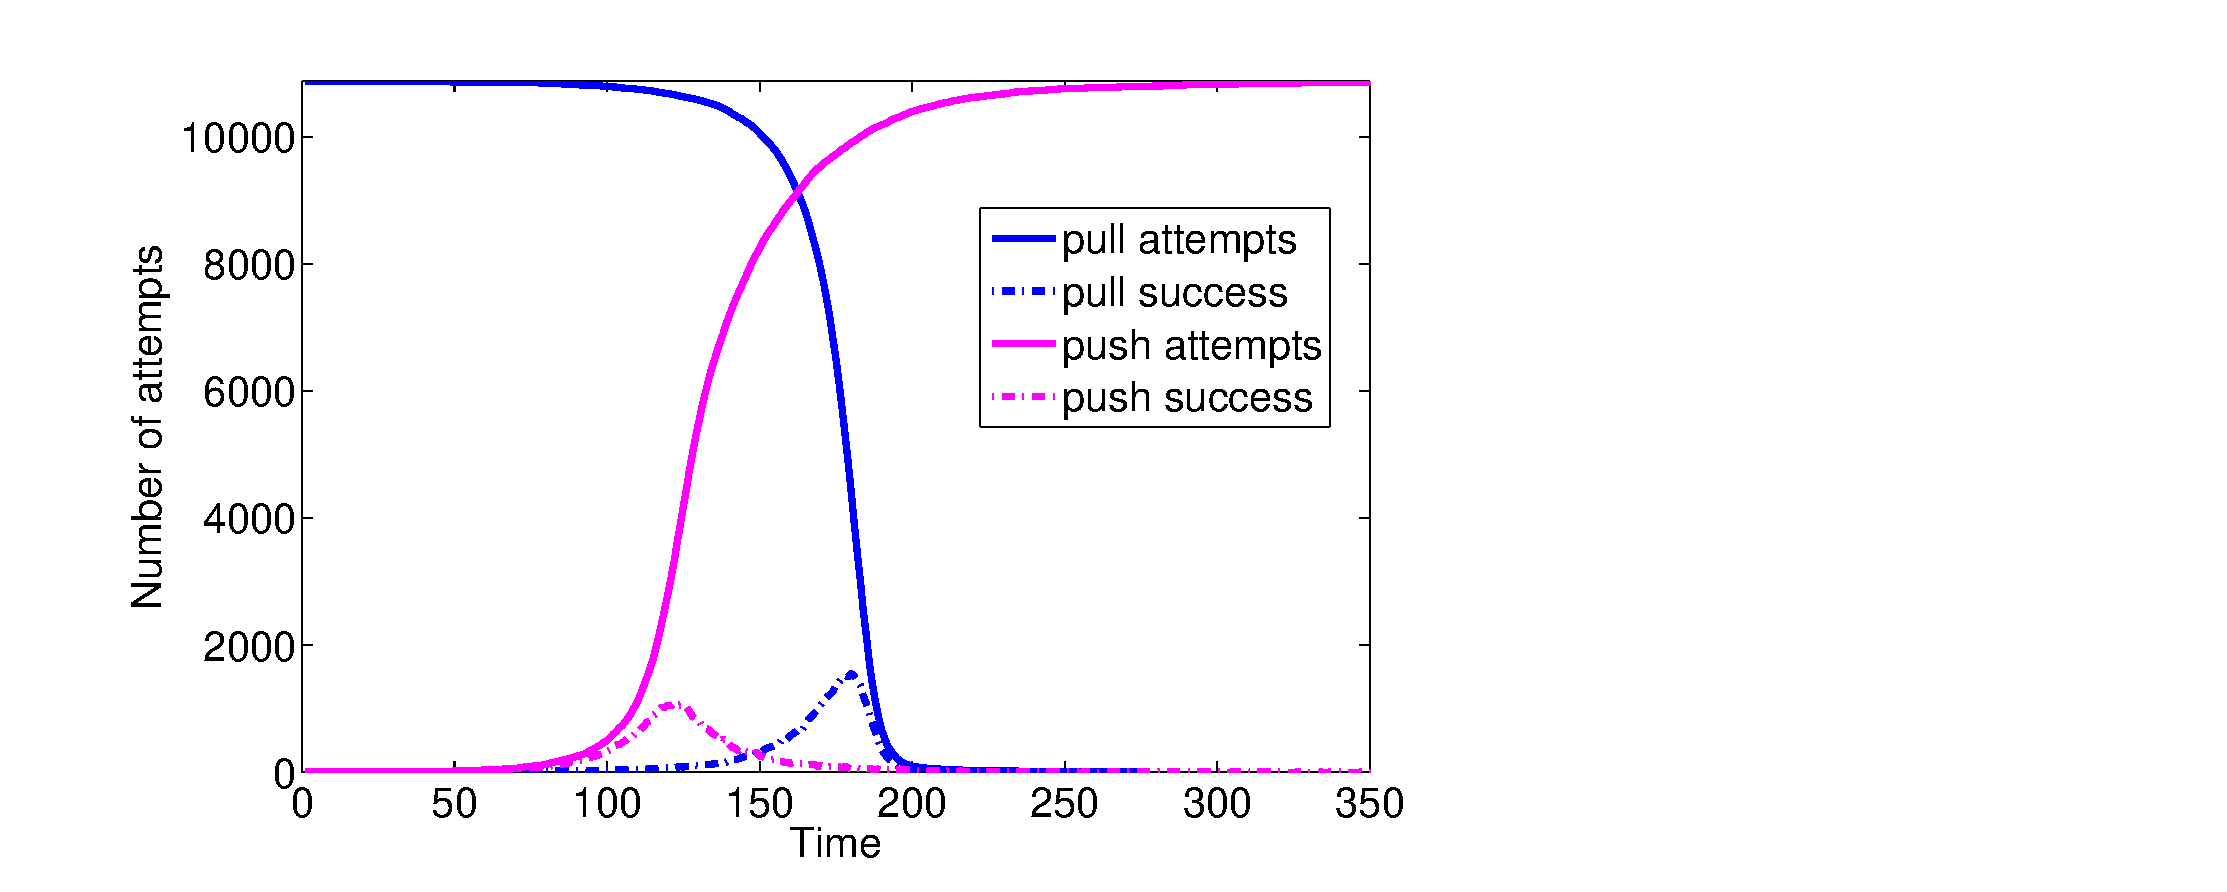
\includegraphics[scale=0.25]{./texfiles/Chapter_3/netsci/figs1/ps_pl_at_su.eps}
\caption{Pull attempts, successful pulls, push attempts, successful pushes versus time for gnutella1 network}
\label{ps_pl_at_su}
\end{figure}

\subsubsection{Strategy-x\%, automatic switch from push to pull}

In this Strategy (X-P-P), the nodes in the system follow $Blind-push$ initially and then switch to $Blind-Pull$ once x\% of the nodes in the system have 
the full message. The algorithm terminates when all the nodes in the system have the full message.

We consider the $Blind-push$ and $Blind-pull$ algorithm on a network and check how efficiently they perform over a broadcast time window. 
In figure ~\ref{ps_pl_at_su} we plot the number of attempts and the number of successful ones for the above two cases on 
  gnutella1 network (described later in this section). 
  This clearly shows pull mechanism  
  performs poorly in the beginning but picks up after a certain percentage of nodes have become senders. We observe just the opposite behavior 
  for push mechanism. Our X-P-P strategy is based on this idea to obtain the best out of both the strategies.

The X-P-P strategy cannot be implemented in a practical setting  because the nodes in the system need to maintain a global information of the percentage of nodes in the 
system having the full message which is difficult in a distributed setting like this.



\subsubsection{A distributed version of X-P-P strategy}
% To obtain a better coverage, we propose a combined strategy which combines $push$ and $pull$ in a practical way and is integrated with the give-up strategy to reduce wastage. We call this the 
% $Push Pull with giveup$ (P-P-G) technique.
% In this strategy,  each node $i$ maintains a counter ($pl\_count_i$, initialized to $0$) and an additional list $l_{i}$ which is initially empty.
% The counter counts
Here, we introduce a new strategy $Push-pull-with-giveup$ (P-P-G) which approximately mimics 
the X-P-P strategy in a distributed setting  and it functions in the following way-
Initially there  is a single node in the system which has the full message. At each time step the sender nodes in the system communicate with one of the nodes 
in their proximity and try to $push$. Among all the other non-sender nodes in the system those which have at least a single packet (i.e., nodes which have participated 
in a message transfer at least once and hence are aware of the broadcast) try to pull. Each node also keeps a local history regarding the number of unsuccessful 
communications it has participated in and once this exceeds a threshold, it `gives-up' and no longer 
participates in the broadcast. Once all the nodes have `given-up', the broadcast terminates.

% \begin{figure}
% \centering
% \includegraphics[scale=0.15]{figs1/xperbt.eps}
% \includegraphics[scale=0.15]{figs1/xperwa.eps}
% \caption{Average broadcast time and wastage versus x for gnutella1,gnutella2 and gnutella3\vspace{-5mm}}
% \label{ps_bt}
% \end{figure}
% \medskip

\subsection{Dynamic topology}
%\vspace{-2mm}
We performed our experiments on gnutella snapshots and on synthetic topologies like complete graph, regular tree, regular graph and random graph. 
A topology specifies the potential neighborhood of a node 
- a node at each time step connects randomly to one of these nodes. A complete graph 
topology would indicate that the 
node can connect to any other node in the network while for other sparser topology it would 
connect only to a subset of them.

%\vspace{-2mm}
%\section{Theoretical analysis}
%\label{theory}
%\noindent
In this section, we first show through numerical simulations that the time to create the first sender, i.e., $T_1$, almost fully determines the overall broadcast time $T^*$. Next, we present an analytical treatment of the push technique for the minimum non-trivial case of $m=k=2$. In particular,  we attempt to compute the expected value of $T_1$ (i.e., $E(T_1)$) which is also supposed to provide an approximate estimation of $E(T^*)$. Finally, we provide pointers for the analytical treatment of the general $m=k$ case.  
We concentrate particularly on the complete graph topology; however, in a later subsection we also analytically study the message propagation for  
$m=k$ on infinite regular trees
\vspace{-3mm}
\subsection{Numerical simulations on complete graph topology}
\vspace{-1mm}



In this section, we give numeric evidence (with analytical support) that the
ratio of the overall broadcast time $T^{\ast }$ and the time to
create the first sender, i.e., $T_{1}$ converges for $n\rightarrow \infty$ to a constant which only depends on $k$. For this purpose we plot in figure~\ref%
{segSizeVsDelay_nrTrans_varyN_Mall_push_pull} the values of $Av(T^{\ast })$
and $Av(T_{1})$ respectively as we vary $n$ where $Av(x)$ represents the average of the quantity $x$ over several simulation runs. We report this distribution for
four different values of $m$ (2, 4, 8 and 16), in each case assuming that
there is only one message segment, i.e., $k=m$. Note that for B-P, the two quantities $Av(T^{\ast })$ and $Av(T_{1})$
exhibit a very similar profile irrespective of the value of $m$ chosen. In the same figure we also plot the function $n^{\frac{k-1}{k}}$ suitably scaled by a constant to show how the theoretical results which we provide in the following sections, closely approximate the numerical simulations. 

\begin{figure}[htbp] 
\centering
\includegraphics[scale=0.36]{figs1/segSizeVsDelay_nrTrans_varyN_Mall_push_pull2.eps}
\caption{$Av(T^*)$ and $Av(T_1)$ versus the number of nodes ($n$). Results are presented for (A) $m=k=2$, (B) $m=k=4$, (C) $m=k=8$, and (D) $m=k=16$. The plots also contain the suitably scaled function $n^{\frac{k-1}{k}}$ for each case.}
\label{segSizeVsDelay_nrTrans_varyN_Mall_push_pull}
\end{figure}
\vspace{-3mm}
\subsection{Performance of B-P in the limit $n\rightarrow \infty$ for complete graph topology}
\vspace{-1mm}


% We compute the expected time to obtain the first sender $E(T_{1})$ as well
% as the expected time $E\left( T^{\ast }\right) $ for broadcasting for a
% message which has $m=2$ packets ($p_{1}$ and $p_{2}$), and $s=1$ segment
% (i.e., the segment has $k=2$ packets). Recall that in push epidemic
% protocol, in each time step, a sender tries to establish a communication
% link with another agent. 
% %In each contact opportunity, only one packet can be
% %transferred from a sender to a receiver.
% As mentioned earlier, we assume only one packet can be transferred from a sender to a receiver in each contact opportunity. 
% 
% At the beginning, a source agent creates a message having 2 packets at time $%
% T_{0}$, this message has to be delivered to all other agents (i.e., $n-1$
% agents) in the network. The number of senders as a function of time is a
% step function and we denote the time of the $i^\textrm{th}$ step by $t_{i}.$ For $i$
% not too large  $\sum\limits_{j=1}^{i}t_{j}$ gives essentially the time $T_{i}$
% when the $i^\textrm{th}$ sender will be created, with the convention that $T_{0}=0$.
% Note that $\sum\limits_{i\geq 1}t_{i}$ is the broadcast time $T^{\ast }$ and 
% $t_{1}$ is the time when the first new sender is created.
% \vspace{-2mm}
% \begin{theorem}
% The random variable $\frac{t_{1}}{\sqrt{n}}$ converges as $n\rightarrow \infty $ to a
% limiting random variable $\tau _{1}$ with density $xe^{-\frac{x^{2}}{2}}$ and
% expectation $E\left( \tau _{1}\right) =\sqrt{\frac{\pi }{2}}.$ Furthermore
% for fixed $i\geq 2$ the random variable $\frac{t_{i}}{\sqrt{n}}$ converges to a
% limiting random variable $\tau _{i}$ and the following recursion holds for the
% expectations: $\frac{E\left( \tau _{i}\right) }{E\left( \tau _{i-1}\right) }%
% =\left( 1-\frac{3}{2i}\right) .$
% \end{theorem}
% \vspace{-2mm}
% \begin{theorem}
% $\frac{T^{\ast }}{\sqrt{n}}$ converges to a limiting random variable $s^{\ast }$ with $%
% E\left( s^{\ast }\right) =\sum\limits_{i=1}^{\infty }E\left( \tau
% _{i}\right) =2\cdot \sqrt{\frac{\pi }{2}}$
% \end{theorem}
% \vspace{-3mm}
% \begin{proof}
% (sketch). We will sketch in the following some of the important steps in the
% proof. For the probability that the first new sender is created at time $t$
% we have%
% \[
% \Pr \left\{ t_{1}=t\right\} =\frac{t-1}{n}\prod\limits_{l=1}^{t-2}\left( 1-%
% \frac{l}{n}\right) ,t\geq 2
% \]%
% Writing $\left( 1-\frac{l}{n}\right) =e^{-\frac{l}{n}+O\left( \frac{l^{2}}{%
% n^{2}}\right) }$we have for the cumulative distribution function 
% \begin{eqnarray*}
% \Pr \left\{ \frac{t_{1}}{\sqrt{n}}\leq x\right\}  &=&\sum\limits_{t\leq x%
% \sqrt{n}}\frac{t-1}{n}\prod\limits_{l=1}^{t-2}\left( 1-\frac{l}{n}\right)  \\
% &=&\sum\limits_{t\leq x\sqrt{n}}\frac{t}{n}e^{-\frac{t^{2}}{2n}+O\left( 
% \frac{t^{3}}{n^{2}}\right) }
% \end{eqnarray*}%
% For $n\rightarrow \infty $, the sum in the last expression converges to $%
% \int\limits_{0}^{x}ye^{-\frac{y^{2}}{2}}dy.$  Hence the limiting density is
% given by $ye^{-\frac{y^{2}}{2}}$ and the expectation by $\int\limits_{0}^{%
% \infty }y^{2}e^{-\frac{y^{2}}{2}}dy=\sqrt{\frac{\pi }{2}}.$ In a similar
% fashion one can obtain the conditional limiting distribution of $\tau _{i}$
% given the value of $b_{i-1}:=\sum\limits_{m=1}^{i-1}m\tau _{m}:$ 
% \[
% \Pr \left\{ \tau _{i}\leq x\right\} =\int\limits_{0}^{x}i\left(
% b_{i-1}+i\tau _{i}\right) e^{-i\left( \tau _{i}b_{i-1}+k\tau
% _{i}^{2}/2\right) }d\tau _{i}
% \]%
% Note that $b_{i}\sqrt{n}$ is the approximate number of nodes with one
% packet up to time $T_{i}.$ By a straightforward but lengthy computation
% using the previous expression for the conditional distribution of $\tau _{i}$
% it can be shown that the recursion $\frac{E\left( \tau _{i}\right) }{E\left(
% \tau _{i-1}\right) }=\left( 1-\frac{3}{2i}\right) $ holds. We will derive
% from this recursion now the expression for $s^{\ast }.$ Clearly we have 
% \[
% E\left( \tau _{i}\right) =\prod\limits_{j\geq 2}^{i}\frac{2j-3}{2j}E\left(
% \tau _{1}\right) 
% \]%
% and hence $s^{\ast }=\left( 1+\sum\limits_{i\geq 2}\prod\limits_{j\geq 2}^{i}%
% \frac{2j-3}{2j}\right) E\left( \tau _{1}\right) .$ Rewriting the product as%
% \[
% \prod\limits_{j\geq 2}^{i}\frac{2j-3}{2j}=\frac{\left( 2\left( i-1\right)
% \right) !}{4^{i-1}\left( \left( i-1\right) !\right) ^{2}i}
% \]%
% we have%
% \[
% s^{\ast }=\left( \sum\limits_{i=0}\frac{\left( 2i\right) !\cdot 2}{%
% 4^{i-1}\left( i!\right) ^{2}\cdot 2\left( i+1\right) }\right) E\left( \tau
% _{1}\right) 
% \]%
% The function 
% \[
% g\left( z\right) :=\sum\limits_{i=0}\frac{\left( 2i\right) !}{%
% 4^{i-1}\left( i!\right) ^{2}\cdot 2\left( i+1\right) }z^{2\left( i+1\right) }
% \]%
% converges for $\left\vert z\right\vert \leq 1$ and satisfies%
% \[
% \frac{d}{dz}g\left( z\right) =z\cdot \frac{d}{dz}\arcsin z=z\cdot \frac{1}{%
% \sqrt{1-z^{2}}}
% \]%
% as can be easily seen by comparing with the Taylor expansion of the right hand side. Hence 
% \[
% g\left( 1\right) =\int\limits_{0}^{1}\frac{z}{\sqrt{1-z^{2}}}dz=1
% \]%
% and $s^{\ast }=2E\left( \tau _{1}\right).$
% \end{proof}
% 
% It is important to note that the above computations can be carried out essentially up to a time $t$ where there are $\sqrt{n}$ senders. The remaining growth is very fast - actually of logarithmic order since several new senders in every time step get produced.
% \vspace{-3mm}
We compute the expected time to obtain the first sender $E(T_{1})$ as well
as the expected time $E\left( T^{\ast }\right) $ for broadcasting for a
message which has $m=2$ packets ($p_{1}$ and $p_{2}$), and $s=1$ segment
(i.e., the segment has $k=2$ packets). Recall that in push epidemic
protocol, in each time step, a sender tries to establish a communication
link with another agent. 
%In each contact opportunity, only one packet can be
%transferred from a sender to a receiver.
As mentioned earlier, we assume only one packet can be transferred from a
sender to a receiver in each contact opportunity.

At the beginning, a source agent creates a message having 2 packets at time $%
T_{0}$, this message has to be delivered to all other agents (i.e., $n-1$
agents) in the network. The number of senders as a function of time is a
step function and we denote the time of the $i^\textrm{th}$ step by $t_{i}.$
For $i$ not too large $\sum\limits_{j=1}^{i}t_{j}$ gives essentially the
time $T_{i}$ when the $i^\textrm{th}$ sender will be created, with the
convention that $T_{0}=0$. Note that $\sum\limits_{i\geq 1}t_{i}$ is the
broadcast time $T^{\ast }$ and $t_{1}$ is the time when the first new sender
is created. \vspace{-2mm} 
\begin{theorem}
The random variable $\frac{t_{1}}{\sqrt{n}}$ converges as $n\rightarrow \infty $ to a
limiting random variable $\tau _{1}$ with density $xe^{-\frac{x^{2}}{2}}$ and
expectation $E\left( \tau _{1}\right) =\sqrt{\frac{\pi }{2}}.$ Furthermore
for fixed $i\geq 2$ the random variable $\frac{t_{i}}{\sqrt{n}}$ converges to a
limiting random variable $\tau _{i}$ and the following recursion holds for the
expectations: $\frac{E\left( \tau _{i}\right) }{E\left( \tau _{i-1}\right) }%
=\left( 1-\frac{3}{2i}\right) .$
\end{theorem}
\vspace{-2mm} 
\begin{theorem}
$\frac{T^{\ast }}{\sqrt{n}}$ converges to a limiting random variable $s^{\ast }$ with $%
E\left( s^{\ast }\right) =\sum\limits_{i=1}^{\infty }E\left( \tau
_{i}\right) =2\cdot \sqrt{\frac{\pi }{2}}$
\end{theorem}
\vspace{-3mm} 
\begin{proof}
(sketch). We will sketch in the following some of the important steps in the
proof. For the probability that the first new sender is created at time $t$
we have%
\[
\Pr \left\{ t_{1}=t\right\} =\frac{t-1}{n}\prod\limits_{l=1}^{t-2}\left( 1-%
\frac{l}{n}\right) ,t\geq 2
\]%
Writing $\left( 1-\frac{l}{n}\right) =e^{-\frac{l}{n}+O\left( \frac{l^{2}}{%
n^{2}}\right) }$we have for the cumulative distribution function 
\begin{eqnarray*}
\Pr \left\{ \frac{t_{1}}{\sqrt{n}}\leq x\right\}  &=&\sum\limits_{t\leq x%
\sqrt{n}}\frac{t-1}{n}\prod\limits_{l=1}^{t-2}\left( 1-\frac{l}{n}\right)  \\
&=&\sum\limits_{t\leq x\sqrt{n}}\frac{t}{n}e^{-\frac{t^{2}}{2n}+O\left( 
\frac{t^{3}}{n^{2}}\right) }
\end{eqnarray*}%
For $n\rightarrow \infty $, the sum in the last expression converges to $%
\int\limits_{0}^{x}ye^{-\frac{y^{2}}{2}}dy.$  Hence the limiting density is
given by $ye^{-\frac{y^{2}}{2}}$ and the expectation by $\int\limits_{0}^{%
\infty }y^{2}e^{-\frac{y^{2}}{2}}dy=\sqrt{\frac{\pi }{2}}.$ In a similar
fashion one can obtain the conditional limiting distribution of $\tau _{i}$
given the value of $b_{i-1}:=\sum\limits_{m=1}^{i-1}m\tau _{m}:$ 
\[
\Pr \left\{ \tau _{i}\leq x\right\} =\int\limits_{0}^{x}i\left(
b_{i-1}+i\tau _{i}\right) e^{-i\left( \tau _{i}b_{i-1}+k\tau
_{i}^{2}/2\right) }d\tau _{i}
\]%
Note that $b_{i}\sqrt{n}$ is the approximate number of nodes with one
packet up to time $T_{i}.$ By a straightforward but lengthy computation
using the previous expression for the conditional distribution of $\tau _{i}$
it can be shown that the recursion $\frac{E\left( \tau _{i}\right) }{E\left(
\tau _{i-1}\right) }=\left( 1-\frac{3}{2i}\right) $ holds. We will derive
from this recursion now the expression for $s^{\ast }.$ Clearly we have 
\[
E\left( \tau _{i}\right) =\prod\limits_{j\geq 2}^{i}\frac{2j-3}{2j}E\left(
\tau _{1}\right) 
\]%
and hence $s^{\ast }=\left( 1+\sum\limits_{i\geq 2}\prod\limits_{j\geq 2}^{i}%
\frac{2j-3}{2j}\right) E\left( \tau _{1}\right) .$ Rewriting the product as%
\[
\prod\limits_{j\geq 2}^{i}\frac{2j-3}{2j}=\frac{\left( 2\left( i-1\right)
\right) !}{4^{i-1}\left( \left( i-1\right) !\right) ^{2}i}
\]%
we have%
\[
s^{\ast }=\left( \sum\limits_{i=0}\frac{\left( 2i\right) !\cdot 2}{%
4^{i-1}\left( i!\right) ^{2}\cdot 2\left( i+1\right) }\right) E\left( \tau
_{1}\right) 
\]%
The function 
\[
g\left( z\right) :=\sum\limits_{i=0}\frac{\left( 2i\right) !}{%
4^{i-1}\left( i!\right) ^{2}\cdot 2\left( i+1\right) }z^{2\left( i+1\right) }
\]%
converges for $\left\vert z\right\vert \leq 1$ and satisfies%
\[
\frac{d}{dz}g\left( z\right) =z\cdot \frac{d}{dz}\arcsin z=z\cdot \frac{1}{%
\sqrt{1-z^{2}}}
\]%
as can be easily seen by comparing with the Taylor expansion of the right hand side. Hence 
\[
g\left( 1\right) =\int\limits_{0}^{1}\frac{z}{\sqrt{1-z^{2}}}dz=1
\]%
and $s^{\ast }=2E\left( \tau _{1}\right).$
\end{proof}

It is important to note that the above computations can be carried out
essentially up to a time $t$ where there are $\sqrt{n}$ senders. The
remaining growth is very fast - actually of logarithmic order since several
new senders in every time step get produced. \vspace{-2mm}
\subsection{A short indication of the results for the general case $m=k$}
\vspace{-1mm}
% Here we present a sketch of the approach to general $m=k$ case. We are
% interested in the waiting time $t_{1}$ for the appearance of the first
% sender. For that, one has to understand how the number of sites which have
% exactly say $l$ packets grows with $t.$ 
% 
% (i) 1-packet carriers grow essentially as $t$ (because the initial sender
% node establishes contacts in most cases, a new node from the pool $n$),
% 
% (ii) 2-packet carriers grow essentially as $\sum\limits^{t}\frac{i}{n}\sim \frac{%
% t^{2}}{2n}$ since at time $i$ the probability to establish contact again from the $i$
% 1-packet carriers is $\frac{i}{n}.$~\footnote{This sum and all the
% following are random variables but for $t$ large enough one can use the
% central limit theorem -- furthermore the fluctuations are small compared to
% the leading term -- can all be worked out nicely and we plan to report this in a forthcoming paper.}
% 
% (iii) 3-packet carriers grow essentially as $\sum\limits^{t}\frac{1}{n}\frac{i^{2}%
% }{2n}\sim \frac{t^{3}}{3\cdot 2\cdot n^{2}}$,
% 
% \bigskip 
% 
% (iv) and finally the $(m-1)$-packet carriers grow essentially as $\frac{t^{m-1}}{\left(
% m-1\right) !n^{m-2}}$
% 
% With this estimation we can now proceed as in the $m=2$ case (conceptually of
% course) since%
% \begin{eqnarray*}
% \Pr \left( t_{1}=t\right)  &\sim &\frac{t^{m-1}}{\left( m-1\right) !n^{m-1}}%
% \prod\limits_{i}^{t}\left( 1-\frac{i^{m-1}}{\left( m-1\right) !n^{m-1}}%
% \right)  \\
% &\sim &\frac{t^{m-1}}{\left( m-1\right) !n^{m-1}}e^{-\frac{t^{m}}{m!n^{m-1}}}
% \end{eqnarray*}%
% From this one sees that $t_{1}$ is of the order $n^{\frac{m-1}{m}}$ .
% 
% More precisely one has for the limiting quantity $\tau
% _{1}=\lim_{n\rightarrow \infty }\frac{t_{1}}{n^{\frac{m-1}{m}}}:$%
% \[
% E\left( \tau _{1}\right) =\int\limits_{0}^{\infty }\frac{y^{m}}{\left(
% m-1\right) !}e^{-\frac{y^{m}}{m!}}dy
% \]%
% and $\tau _{1}$ has density $\frac{y^{m-1}}{\left( m-1\right) !}e^{-\frac{%
% y^{m}}{m!}}.$
Here we present a sketch of the approach to general $m=k$ case. We are
interested in the waiting time $t_{1}$ for the appearance of the first
sender. For that one has to understand how the number of sites which have
exactly say $l$ packets grows with $t.$

(i) 1-packet carriers grow essentially as $t$ (because the initial sender
node establishes contacts in most cases a new node from the pool $n$),

(ii) 2-packet carriers grow essentially as $\sum\limits^{t}\frac{i}{n}\sim 
\frac{t^{2}}{2n}$ since at time $i$ the probability to establish contact
again from the $i$ 1-packet carriers is $\frac{i}{n}.$~\footnote{%
This sum and all the following are random variables but for $t$ large enough
one can use the central limit theorem -- furthermore the fluctuations are
small compared to the leading term -- can all be worked out nicely and we
plan to report this in a forthcoming paper.}

(iii) 3-packet carriers grow essentially as $\sum\limits^{t}\frac{1}{n}\frac{%
i^{2}}{2n}\sim \frac{t^{3}}{3\cdot 2\cdot n^{2}}$,

\bigskip

(iv) and finally the $(m-1)$-packet carriers grow essentially as $\frac{%
t^{m-1}}{\left( m-1\right) !n^{m-2}}$

With this estimation we can now proceed as in the $m=2$ case (conceptually
of course) since%
\begin{eqnarray*}
\Pr \left( t_{1}=t\right) &\sim &\frac{t^{m-1}}{\left( m-1\right) !n^{m-1}}%
\prod\limits_{i}^{t}\left( 1-\frac{i^{m-1}}{\left( m-1\right) !n^{m-1}}%
\right) \\
&\sim &\frac{t^{m-1}}{\left( m-1\right) !n^{m-1}}e^{-\frac{t^{m}}{m!n^{m-1}}}
\end{eqnarray*}%
From this one sees that $t_{1}$ is of the order $n^{\frac{m-1}{m}}$ .

More precisely one has for the limiting quantity $\tau
_{1}=\lim_{n\rightarrow \infty }\frac{t_{1}}{n^{\frac{m-1}{m}}}:$%
\[
E\left( \tau _{1}\right) =\int\limits_{0}^{\infty }\frac{y^{m}}{\left(
m-1\right) !}e^{-\frac{y^{m}}{m!}}dy 
\]%
and $\tau _{1}$ has density $\frac{y^{m-1}}{\left( m-1\right) !}e^{-\frac{%
y^{m}}{m!}}.$

\subsection{Theoretical analysis for infinite regular trees}   
In this section we study the characteristics of message propagation with $m=k$ on
infinite regular trees. The same analysis provided here holds mutatis
mutandis for trees generated by branching processes with Poisson offspring
distribution.

We start with the case of $d$ $-$ regular trees for $d\geq 3$ with a
distinguished root index $0$ which acts as the initial sender. For
simplicity we give the root an out-degree of $d-1$ by attaching a virtual
``mother vertex'' to the root which is also a sender but has only one
offspring and is not counted in the estimation of sender nodes (this helps us avoid
handling the initial steps (when only the root is having the message)
differently from the later steps). Let $A_{l}\left( t\right) ,$ $0\leq l<m,$
be the number of nodes on the tree which have exactly $l$ packets at time $t
$ and have a direct communication link to one of the sender nodes at time $t$. Note that each of the so defined nodes has exactly one connection to a
sender node due to the tree structure and the initial condition of having
just one sender at the beginning. We get the following linear exact
recursion for the expectation $a_{l}\left( t+1\right) :=\mathbb{E}\left(
A_{l}\left( t+1\right) \right) $ at time $t+1:$%
\begin{eqnarray*}
a_{l}\left( t+1\right)  &=&\frac{k-1}{k}a_{l}\left( t\right) +\frac{1}{k}%
a_{l-1}\left( t\right) ,1\leq l\leq m-1 \\
a_{0}\left( t+1\right)  &=&\frac{k-1}{k}a_{m-1}\left( t\right) +\frac{k-1}{k}%
a_{0}\left( t\right) 
\end{eqnarray*}%
Note that for the expected number of sender nodes $s_{t}$ at time $t$ we
have 
\[
s_{t}=\sum\limits_{t^{\prime }<t}\frac{1}{k}a_{m-1}\left( t^{\prime }\right) 
\]
The asymptotic rate of growth of the variables $\left\{ a_{i}\left( t\right)
\right\} $ as well as $s_{t}$ is entirely determined by the value of the
largest eigenvalue of the associated transition matrix. The maximal
eigenvalue of the associated characteristic polynomial is given by 
\[
\lambda _{\max }=\frac{k-1}{k}+\left( \frac{k-1}{k}\left( \frac{1}{k}\right)
^{m-1}\right) ^{\frac{1}{m}}=\frac{k-1+\left( k-1\right) ^{1/m}}{k}
\]%
We study the maximum of the function $\frac{x-1+\left( x-1\right) ^{1/m}}{x}$
for $x>2.$ Setting the derivative to zero gives the condition 
\[
\left( x-1\right) ^{m-1}=\left( \frac{m-1}{m}x-1\right) ^{m},x>2
\]%
We therefore get
\[
\left( 1-\frac{x}{m\left( x-1\right) }\right) ^{m-1}\cdot \left( x-1-\frac{%
x}{m}\right)=1 
\]%
and in the limit $m\rightarrow \infty $ we obtain%
\[
\left( x-1\right) e^{-\frac{x}{x-1}}=1
\]%
Note that the whole computation holds also for the case of a Poisson
offspring distribution with expectation $k-1.$
\medskip
\section{Experiment on different network topologies}
\label{suggestions}
%\vspace{-1mm}
\noindent
In this section we systematically study the effect of topology of the underlying contact network on the broadcast time and wastage and come up with some suggestions which we 
feel will be helpful while designing networks.  
%First we analyze the B-P algorithm on complete graph topology and observe that the broadcast time scales 
%as $n^{\frac{k-1}{k}}$. 
We first analyze B-P algorithm on different topologies like regular graph, regular tree and random graph. In particular, we wish to 
check whether the average degree ($d$) of the underlying contact network influences the 
 performance metrics. 
 %Since it is difficult to interpolate through every value of $d$ for a real network, we perform our simulations on the synthetic networks.
 In the later part of this section we make a comparative study of different broadcast strategies (discussed in section ~\ref{algorithm_outline}) and also
 reinspect into their sparser variants to identify the effect of lowering the value of $d$ 
 through removal of edges without hampering network connectivity.
\subsection{Blind push on different topologies} 
\if{0}
%\vspace{-5mm}
\subsection{Blind push on complete graph}
% \vspace{-2mm}
 We analyze the performance of B-P on complete graph topology. A complete graph topology indicates that a node in the system can communicate with any other node. 
 We provide numeric evidence (with analytical support) that the
ratio of the overall broadcast time $T^{\ast }$ and the time to
create the first sender, i.e., $T_{1}$ converges to a constant which only depends on $k$. 
For this purpose we plot in figure~\ref%
{segSizeVsDelay_nrTrans_varyN_Mall_push_pull} the values of $Av(T^{\ast })$
and $Av(T_{1})$ respectively as we vary $n$ where $Av(y)$ represents the average of the quantity $y$ over several simulation runs. We report this distribution for
four different values of $m$ (2, 4, 8 and 16), in each case assuming that
there is only one message segment, i.e., $k=m$. Note that for B-P, the two quantities $Av(T^{\ast })$ and $Av(T_{1})$
exhibit a very similar profile irrespective of the value of $m$ chosen. In the same figure we also plot the function $n^{\frac{k-1}{k}}$ suitably scaled by a constant to show how the theoretical results which we provide next, closely approximate the numerical simulations. 

\begin{figure}[htbp] 
\centering
\includegraphics[scale=0.36]{./texfiles/Chapter_3/netsci/figs1/segSizeVsDelay_nrTrans_varyN_Mall_push_pull2.eps}
\caption{$Av(T^*)$ and $Av(T_1)$ versus the number of nodes ($n$). Results are presented for (A) $m=k=2$, (B) $m=k=4$, (C) $m=k=8$, and (D) $m=k=16$. The plots also contain the suitably scaled function $n^{\frac{k-1}{k}}$ for each case.}
\label{segSizeVsDelay_nrTrans_varyN_Mall_push_pull}
\end{figure}
%\subsection{Performance of B-P in the limit $n\rightarrow \infty$ for complete graph topology}
\subsubsection{Analytical estimate}

We initially start by considering a message which has $m=2$ packets and $s=1$ segment (i.e., the segment has $k=2$ packets). We compute the expected time to 
obtain the first sender\footnote{
Note that first sender refers to the first node (other than the initiator) which 
receives the full message during the broadcast phase.
} $E(T_1)$. 
%and the expected time for broadcast $E(T^{\ast})$. 
It is important to note that $T_1$ is an indicator for the total broadcast time $T^*$ since the remaining growth is of logarithmic order as after creation of the first sender, 
several senders are produced at regular interval thus speeding
up the transfer exponentially. 
We provide an outline of the analytical expression, the detail is more involved and is ommitted in the interest of space. 
 
At time $T_0$, an initiator is created and it has the full message. Since we are considering 
message size of $2$ so the first sender can be created at least in 2 time steps which is possible
 if the same node is selected in these two time steps. Next we calculate 
$Pr\{T_1=t\}$ that is the probability that the  first sender is created at time $t$. This implies
for the $t-1$ time steps, only the nodes without any packets are selected and at time step $t$ one 
from the $t-1$ nodes are selected. So we have


\begin{align*}
\Pr \{ T_{1}=t\} &=(1-\frac{1}{n})(1-\frac{2}{n})(1-\frac{3}{n})...(1-\frac{t-2}{n})(\frac{t-1}{n}) \\ 
 &=\frac{t-1}{n}\prod\limits_{l=1}^{t-2}( 1-%
\frac{l}{n}) ,t\geq 2
\end{align*}
Infact if $\tau_i$ represent the time to create the first sender then it can be shown that the recursion  $\frac{E\left( \tau _{i}\right) }{E\left(
\tau _{i-1}\right) }=\left( 1-\frac{3}{2i}\right) $ holds. 
From this one can show that $E(T^*)=2*E(T_1)$
\if{0}
Writing $\left( 1-\frac{l}{n}\right) =e^{-\frac{l}{n}+O\left( \frac{l^{2}}{%
n^{2}}\right) }$we have for the cumulative distribution function 
\begin{eqnarray*}
\Pr \left\{ \frac{t_{1}}{\sqrt{n}}\leq x\right\}  &=&\sum\limits_{t\leq x%
\sqrt{n}}\frac{t-1}{n}\prod\limits_{l=1}^{t-2}\left( 1-\frac{l}{n}\right)  \\
&=&\sum\limits_{t\leq x\sqrt{n}}\frac{t}{n}e^{-\frac{t^{2}}{2n}+O\left( 
\frac{t^{3}}{n^{2}}\right) }
\end{eqnarray*}%
For $n\rightarrow \infty $, the sum in the last expression converges to $%
\int\limits_{0}^{x}ye^{-\frac{y^{2}}{2}}dy.$  Hence the limiting density is
given by $ye^{-\frac{y^{2}}{2}}$ and the expectation by $\int\limits_{0}^{%
\infty }y^{2}e^{-\frac{y^{2}}{2}}dy=\sqrt{\frac{\pi }{2}}.$
%\vspace{-2mm}
\fi

Generalizing for case where $k$ $>$ 2, we calculate the time to create the first sender $T_1$. To do it we look into how the number of nodes with exactly $l$ packets (say)
grow with $t$ ($l$ varies from $1$ to $k$ -1). 
We can show that the number of nodes with $l$ packets 
 grow  as $\frac{%
t^{l}}{\left( l\right) !n^{l-1}}$

With this estimation we can now proceed in the same way as we did in case of $k=2$ case and show that 
\begin{eqnarray*}
\Pr \left( T_{1}=t\right) &\sim &\frac{t^{k-1}}{\left( k-1\right) !n^{k-1}}%
\prod\limits_{i}^{t}\left( 1-\frac{i^{k-1}}{\left( k-1\right) !n^{k-1}}%
\right) \\
&\sim &\frac{t^{k-1}}{\left( k-1\right) !n^{k-1}}e^{-\frac{t^{k}}{k!n^{k-1}}}
\end{eqnarray*}%

From the above probability distribution of $T_{1}$ we calculate $E(T_{1})=\sum t*\frac{t^{k-1}}{\left( k-1\right) !n^{k-1}}e^{-\frac{t^{k}}{k!n^{k-1}}}$
and through a lengthy calculation can show that $E(T_{1})$ is of the order $n^{\frac{k-1}{k}}$.
 
%  It is important to note that $T_1$ is an indication for the total broadcast time $T^*$ since the remaining growth is very fast - actually of 
%  logarithmic order since several senders at every time step get produced.
 \vspace{-2mm}
 \fi
%\subsection{Blind push on sparser topologies}
%\vspace{-2mm}
The results of B-P on complete graph are similar to the ones provided in section \ref{res_complete}, hence we concentrate on the sparser topologies. 
In specific, we empirically analyze the B-P algorithm on regular-tree, regular-graph and random-graph. For each topology we consider $n=200$, $m = 4$ and $k=2$.
Note that here we consider that the message has $2$ segments and each segment has $k=2$ packets. 
We then vary the average degree $d$ for each of these networks and check how broadcast delay and wastage depend on it. Remarkably, for each of these topologies 
- regular tree (figure ~\ref{DiffTopologyTree_N200_varyD_push_pull}), regular graph (figure ~\ref{DiffTopologyGraph_N200_varyD_push_pull}) and random graph 
(figure ~\ref{DiffTopologyGnp_N200_varyD_push_pull}), one can observe that there is a critical value of $d$ for which we obtain minimum broadcast delay and 
wastage.
% Here, we assume a finite regular tree topology for $G$ where $n = 200$, $m = 4$ and $k=2$. We vary the degree $d$ of the tree from values ranging from 2 to 10 (see figure~\ref{DiffTopologyTree_N200_varyD_push_pull}). An important observation is that both the broadcast time and the broadcast wastage become significantly low at a critical value of $d$. In fact, for this value of $d$, the metrics of interest reach their minima for B-P technique. 
% \vspace{-3mm}
% \subsection{Regular graph}
% 
% Here, we assume a regular graph topology for $G$ where $n = 200$, $m = 4$ and $k=2$. Once again, we vary the degree $d$ of the graph from values ranging from 1 to 200 (see figure~\ref{DiffTopologyGraph_N200_varyD_push_pull}). The same observation that both the broadcast time and the broadcast wastage become significantly low for a certain value of $d$ also hold in this case and for this value of $d$ the broadcast time is found to scale as $\log{(n)}$. Again at this value of $d$, the metrics of interest reach their minima for the B-P technique.  
% 
% % \begin{figure}
% % \centering
% % 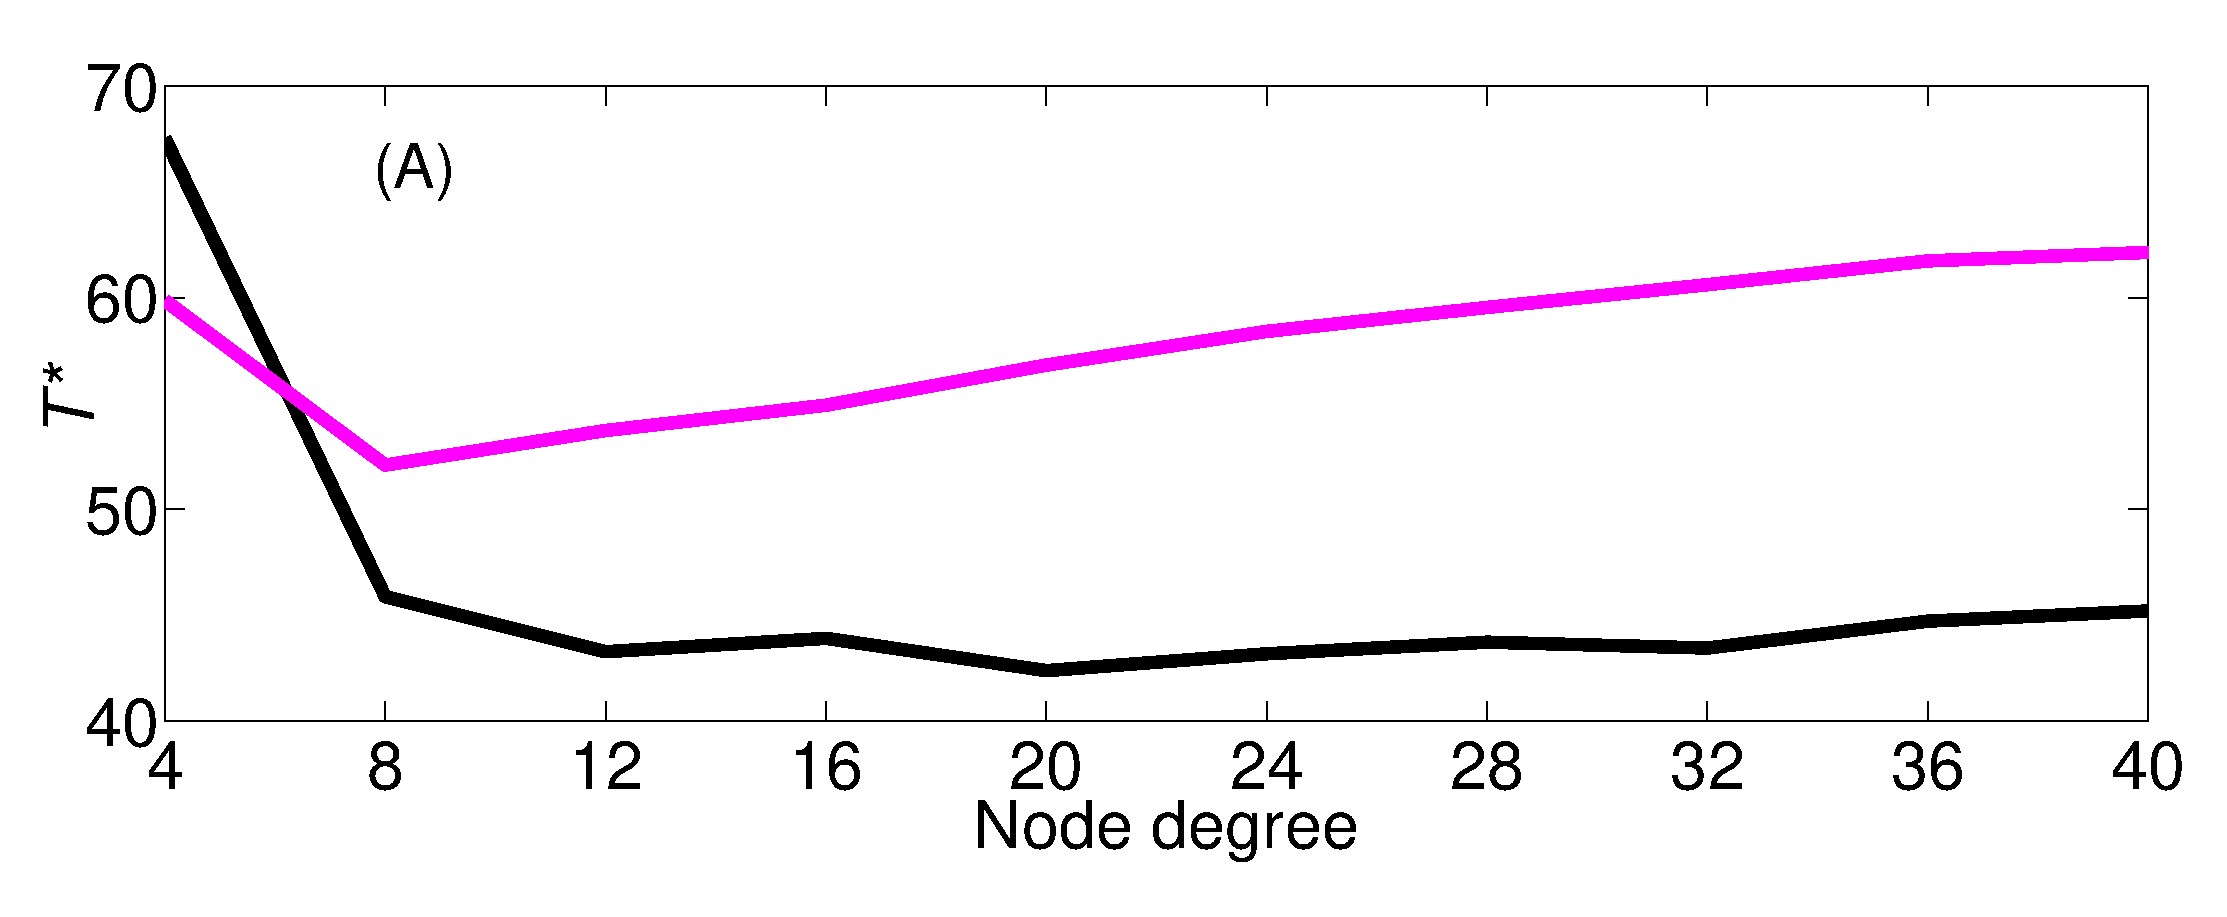
\includegraphics[scale=0.15]{figs1/random_graphs_delay.eps}
% % 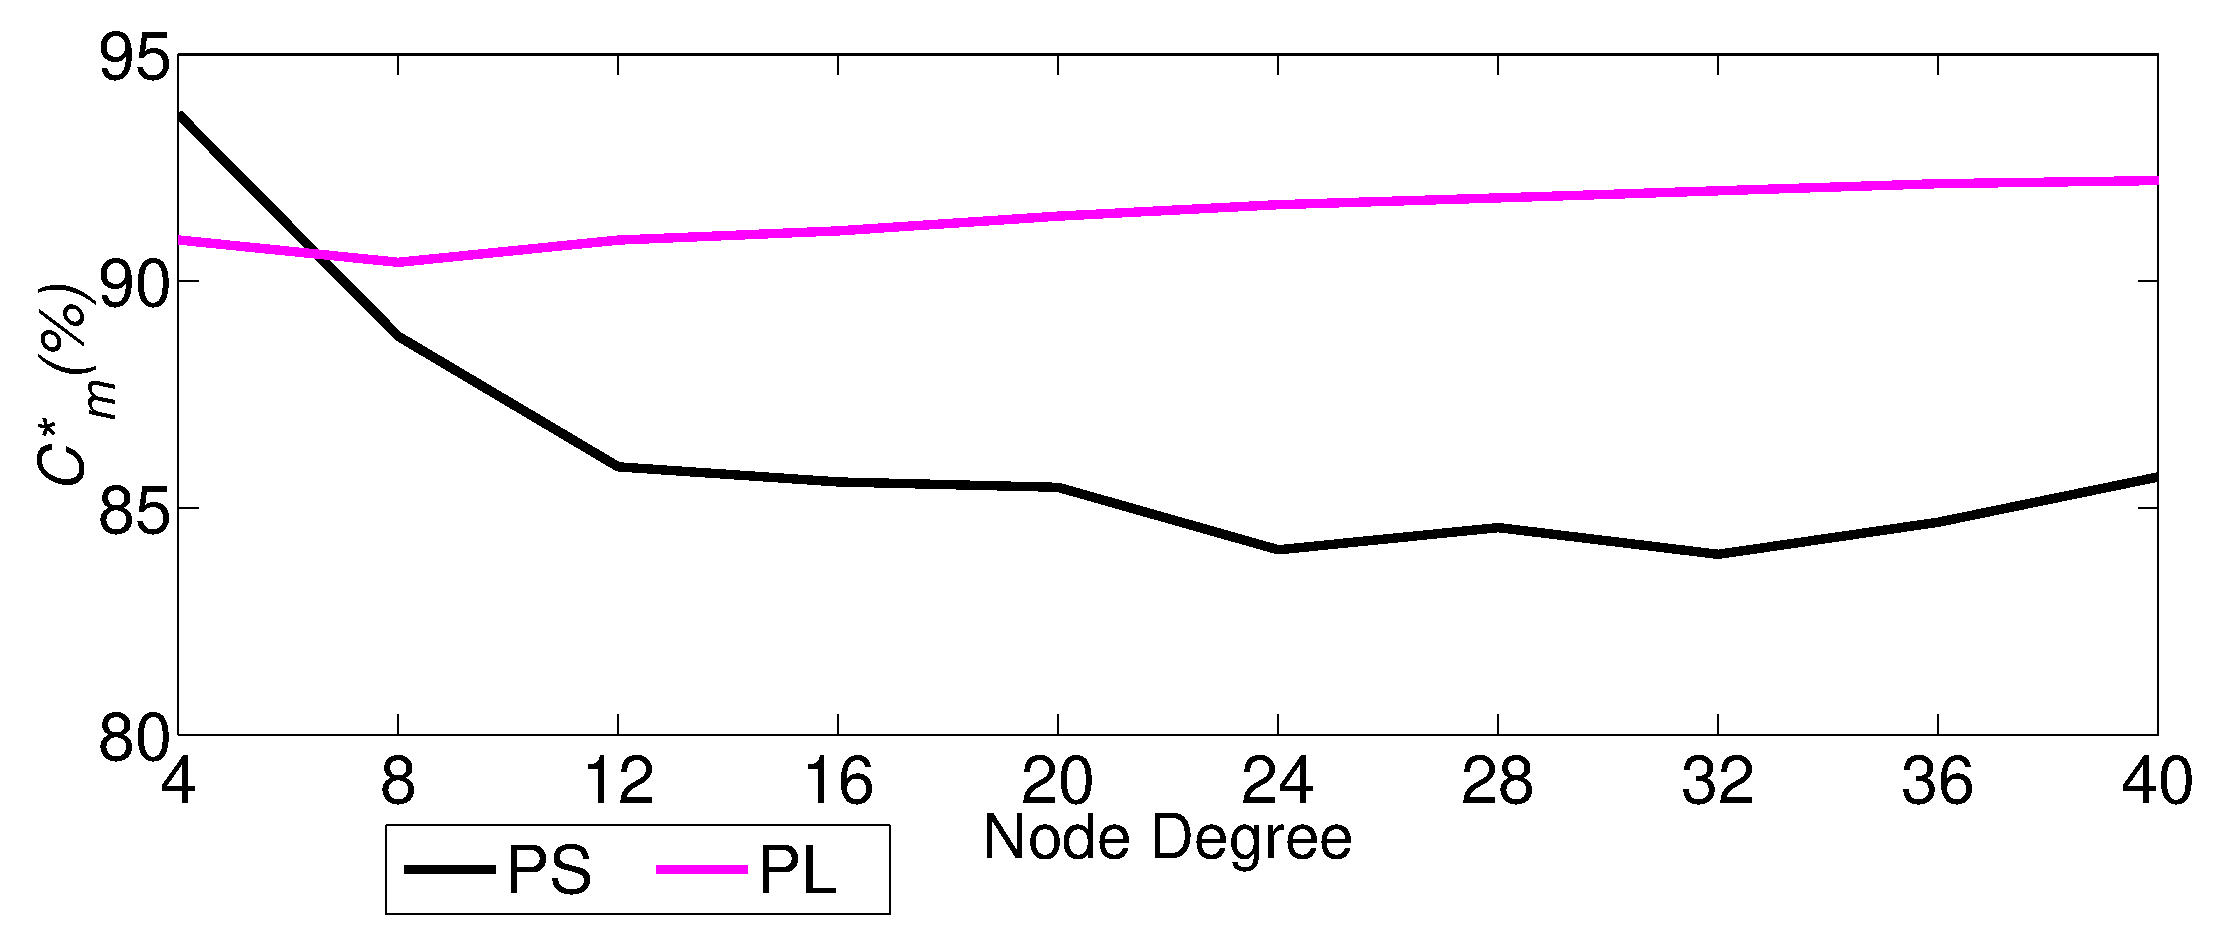
\includegraphics[scale=0.15]{figs1/random_graphs_wastage.eps}
% % \caption{(A) Broadcast time and (B) broadcast wastage versus average degree for B-P . The parameters values are $n=200, m=4, k=2$.\vspace{-3mm}}
% % \label{DiffTopologyGnp_N200_varyD_push_pull}
% % \end{figure}
% % 
% % \begin{figure}
% % \centering
% % \includegraphics[scale=0.4]{diagrams/M2final/DiffTopologyRegularTree_delay_cost_N200_m4_k2_varyD_ps_plRes.eps}
% % \caption{(A) Broadcast time and (B) broadcast wastage versus different values of $d$ for B-P. The parameters values are $n=200, m=4, k=2$.\vspace{-3mm}}
% % \label{DiffTopologyTree_N200_varyD_push_pull}
% % \end{figure}
% \vspace{-3mm}
%  \subsection{Random graph}
%  Here, we assume a random graph topology $G(n, p)$ where $n = 200$, $m = 4$ and $k=2$. Here we vary the probability $p$ of connection (equivalently the average degree $d$) from values ranging from 0.02 to 0.2 (the value of $d$ equivalently varies from 4 to 40) (see figure~\ref{DiffTopologyGnp_N200_varyD_push_pull}). Once again the same observation that both the broadcast time and the broadcast wastage become significantly low for a certain value of $d$ also hold in this case and for this value of $p$ the broadcast time is found to scale as $\log{(n)}$. 
% 
% Thus irrespective of the topology we are able to find a critical value of average degree for the network for which the dynamics becomes as fast as epidemic routing 
% even for the blind push case. Therefore for designing a topology for a network we recommend that the designers look for such a critical value of average degree 
% for which the dynamics becomes fast.
% 
% % \begin{figure}
% % \centering
% % 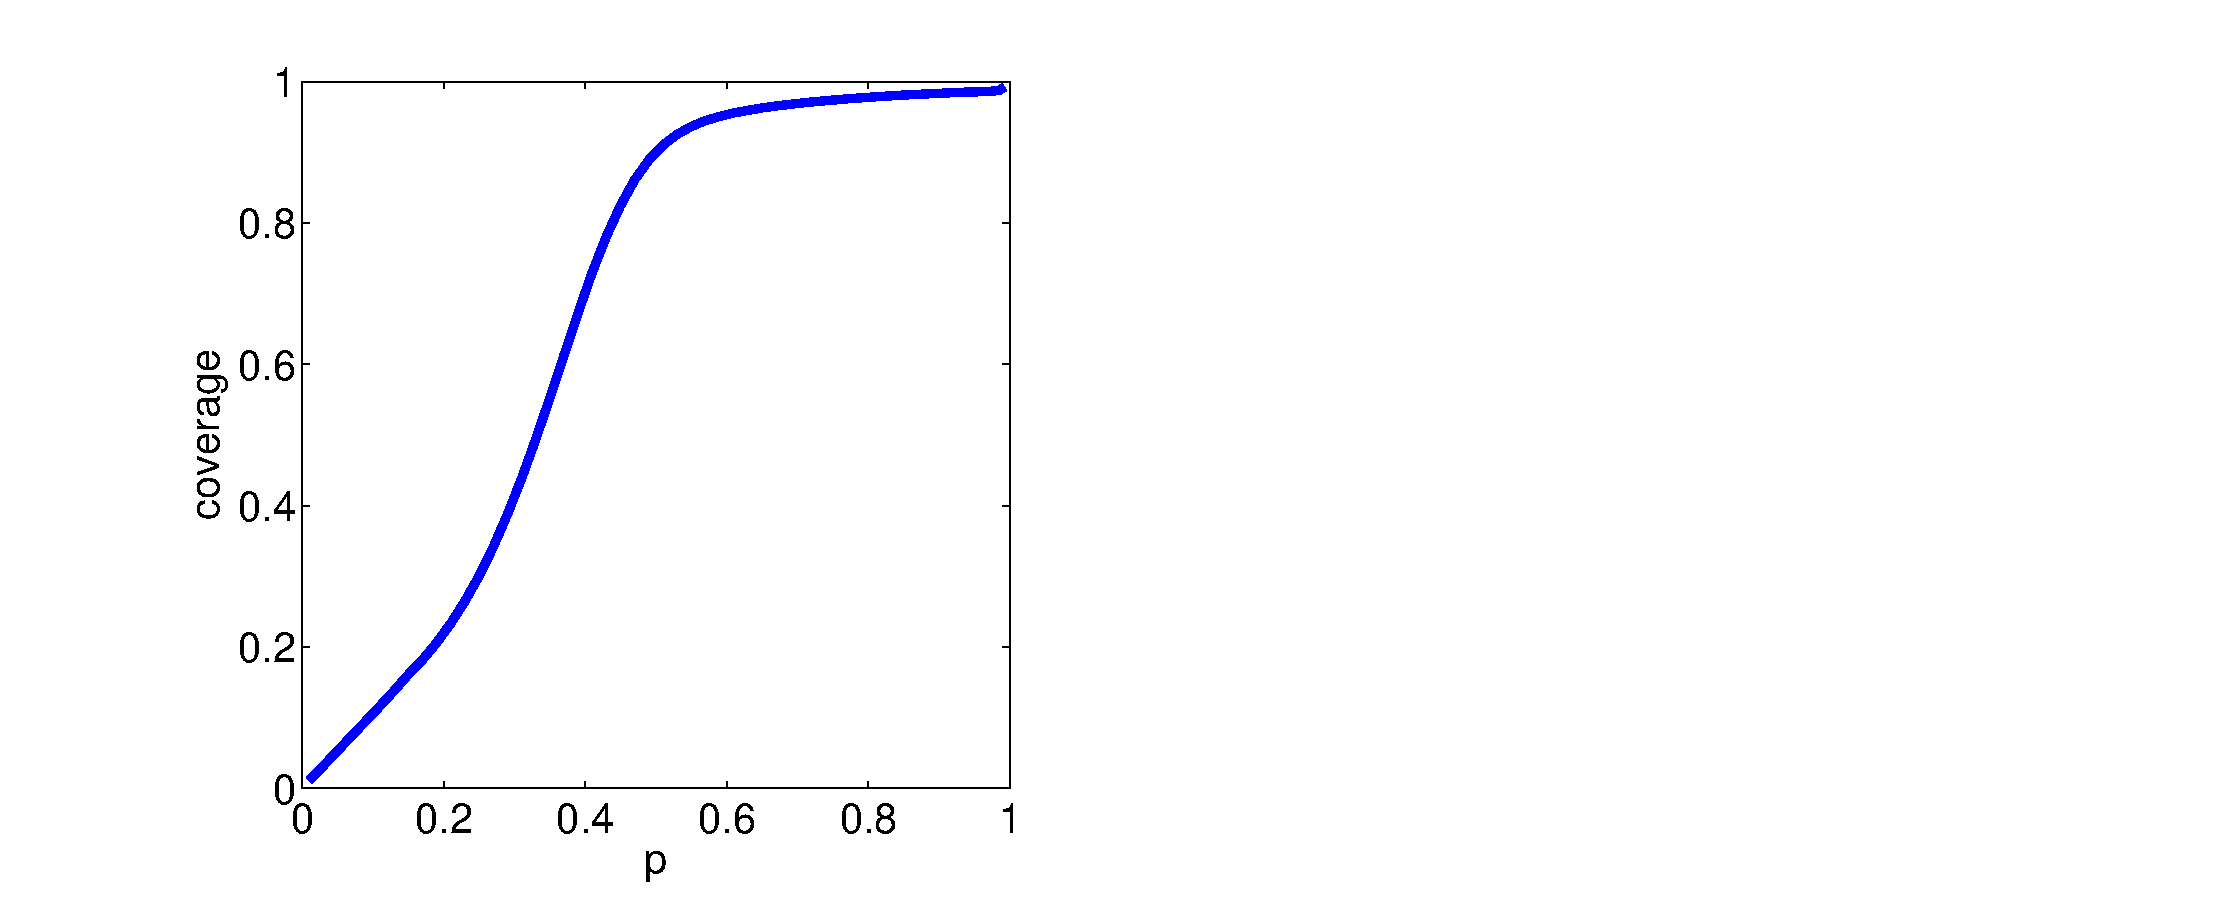
\includegraphics[scale=0.4]{figs1/pvsco.eps}
% % \caption{$p$ versus coverage for gnutella1 network, broadcast technique -- P-P-G \vspace{-3mm}}
% % \label{pcov}
% % \end{figure}

% Since the value of the critical average degree is found to be on the lower side, we performed simulations on sparser variants of the real traces (used previously) 
% and observed that broadcast time reduces even for the B-P. We considered each gnutella snapshot and randomly removed some of the edges such that the 
% network remains connected while producing a sparser variant. From figure ~\ref{gnutellasparse} we observe that the broadcast time reduces significantly 
% in case of the sparser variants in comparison to the original network. 
% Hence, while designing a network it is advisable to keep the network sparse rather than creating unnecessary connections between the nodes. 
% This, as our results indicate, should lead to a faster dissemination of messages.
% \begin{figure}
% \centering
% \includegraphics[scale=0.15]{figs1/random_graphs_delay1.eps}
% \includegraphics[scale=0.15]{figs1/random_graphs_wastage1.eps}
% \caption{(A) Broadcast time and (B) broadcast wastage versus average degree for B-P . The parameters values are $n=200, m=4, k=2$.\vspace{-3mm}}
% \label{DiffTopologyGnp_N200_varyD_push_pull}
% \end{figure}

\begin{figure}
\centering
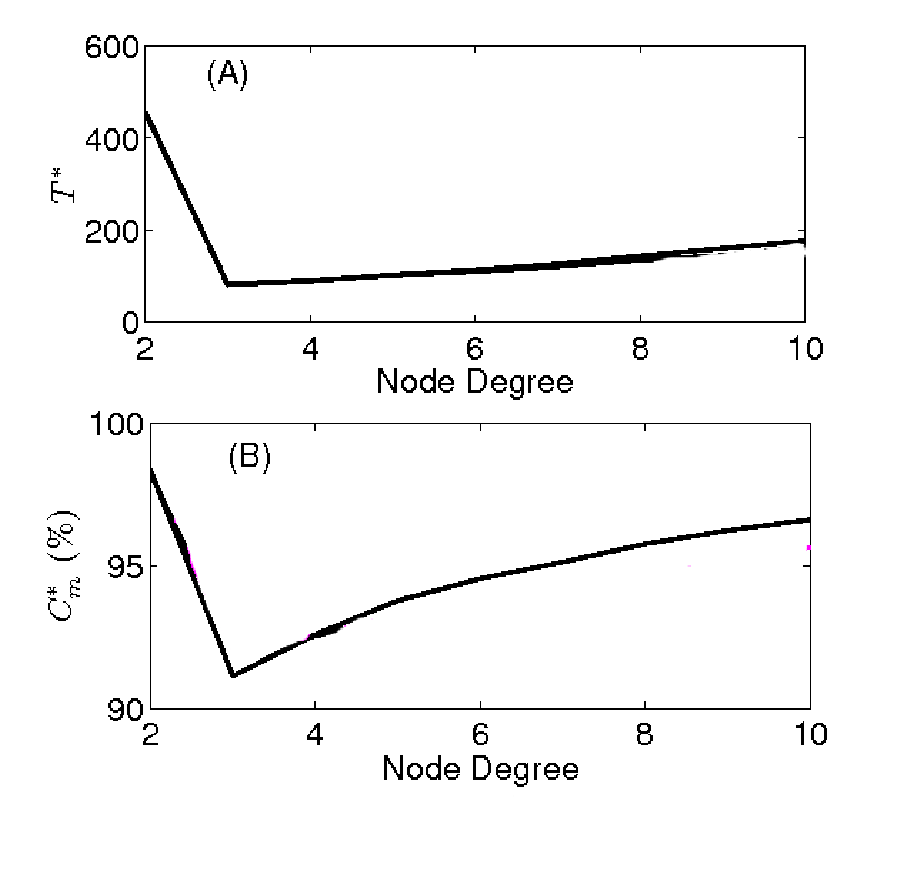
\includegraphics[scale=0.4]{./texfiles/Chapter_3/netsci/figs1/DiffTopologyRegularTree_delay_cost_N200_m4_k2_varyD_ps_plRes1.eps}
\caption{(A) Broadcast time and (B) broadcast wastage versus different values of $d$ for B-P. The parameters values are $n=200, m=4, k=2$.}
\label{DiffTopologyTree_N200_varyD_push_pull}
\end{figure}
%\subsection{Random graph}
%In this section, we assume a random graph topology $G(n, p)$ where $n = 200$, $m = 4$ and $k=2$. Here we vary the probability $p$ of connection (equivalently the average degree $d$) from values ranging from 0.02 to 0.2 (the value of $d$ equivalently varies from 4 to 40) (see figure~\ref{DiffTopologyGnp_N200_varyD_push_pull}). Once again the same observation that both the broadcast time and the broadcast wastage become significantly low for a certain value of $d$ also hold in this case and for this value of $p$ the broadcast time is found to scale as $\log{(n)}$. 

\begin{figure}
\centering
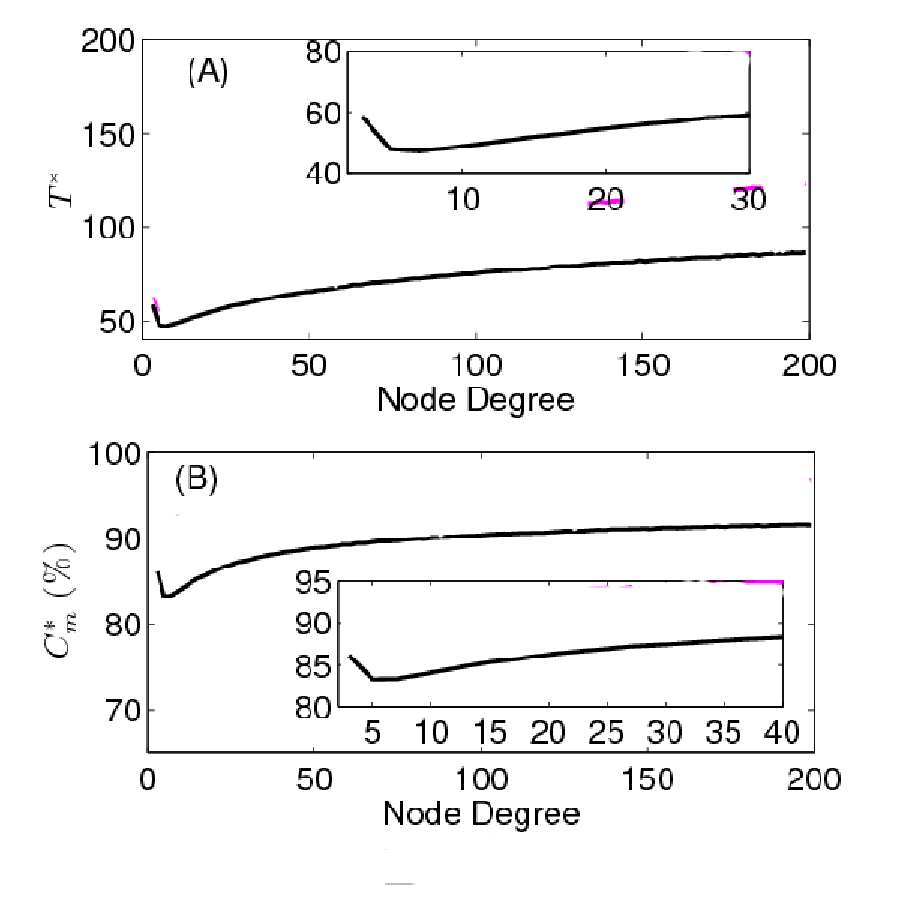
\includegraphics[scale=0.35]{./texfiles/Chapter_3/netsci/figs1/DiffTopology_varyN200_varyD_push_pullRes_m4_k21.eps}
\caption{(A) Broadcast time and (B) broadcast wastage versus different values of $d$ for B-P technique. The parameters values are $n=200, m=4, k=2$. The inset in both the figures show the metrics of interest for the first few values of $d$ to indicate the critical $d$ more appropriately.}
\label{DiffTopologyGraph_N200_varyD_push_pull}
\end{figure}



% \begin{figure}
% \centering
% 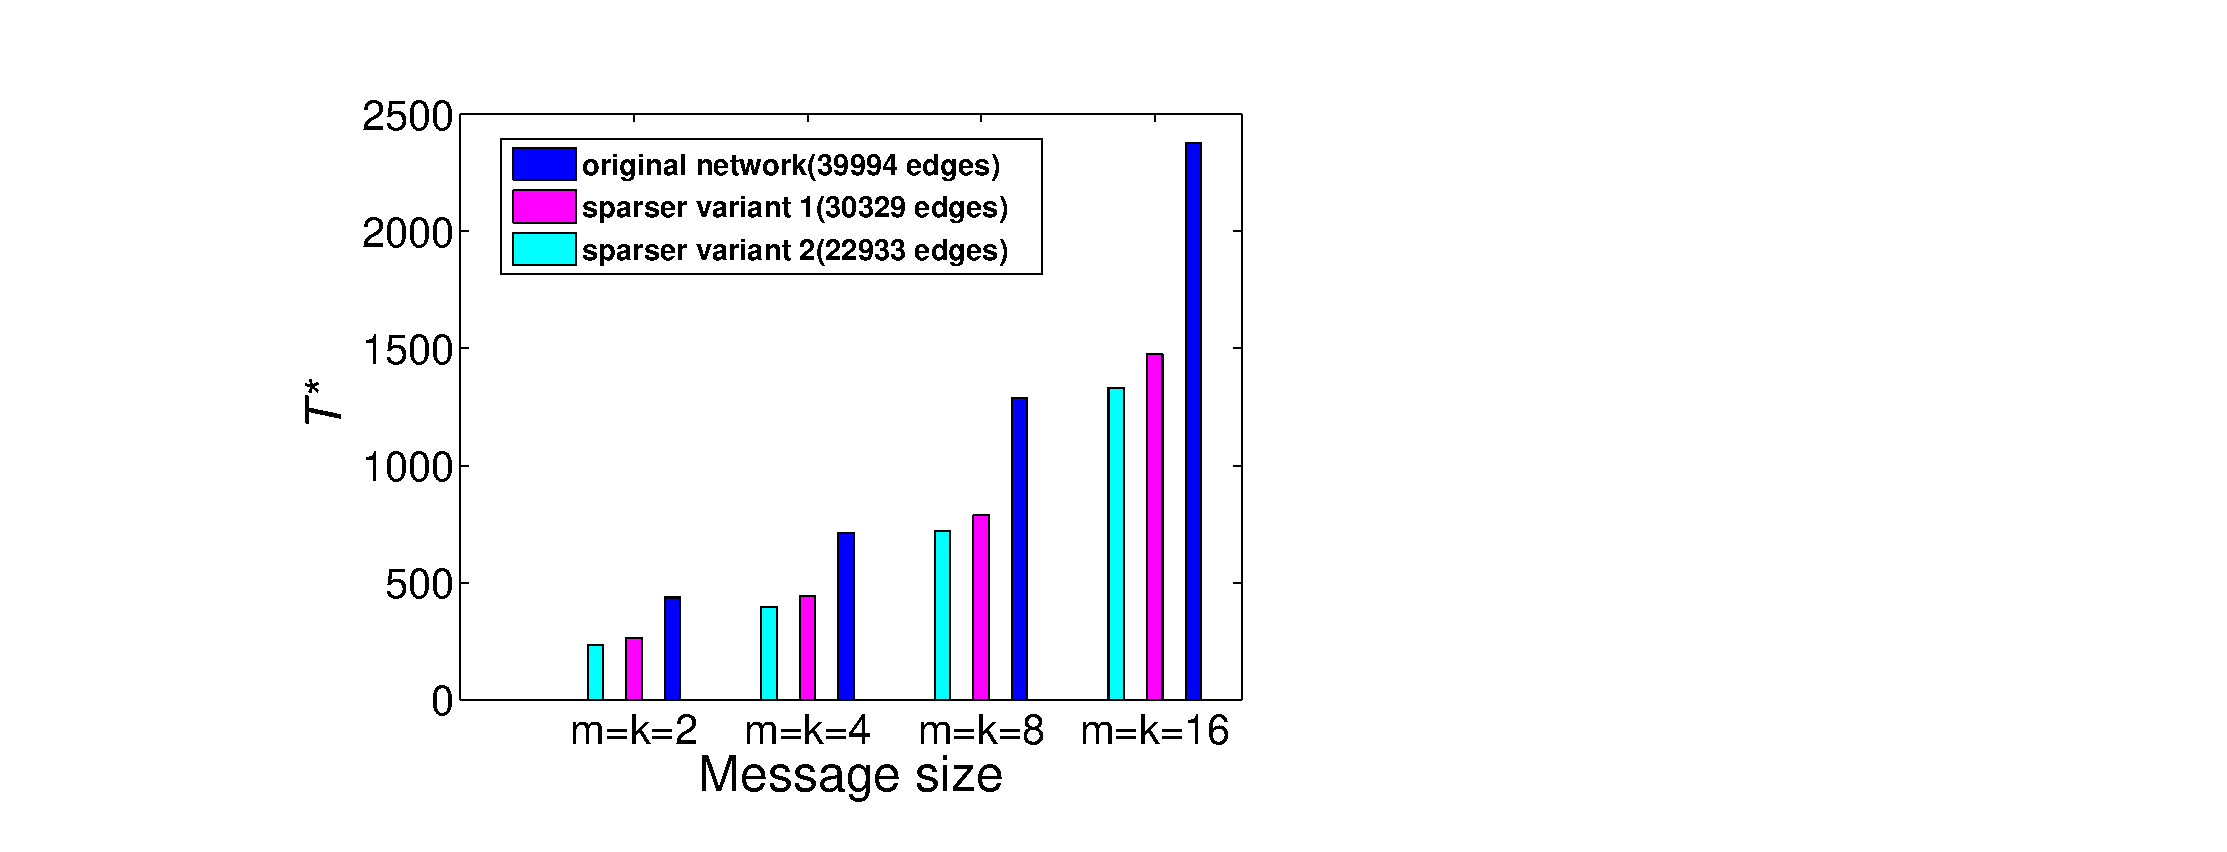
\includegraphics[scale=0.25]{figs1/gnutella1.eps}
% 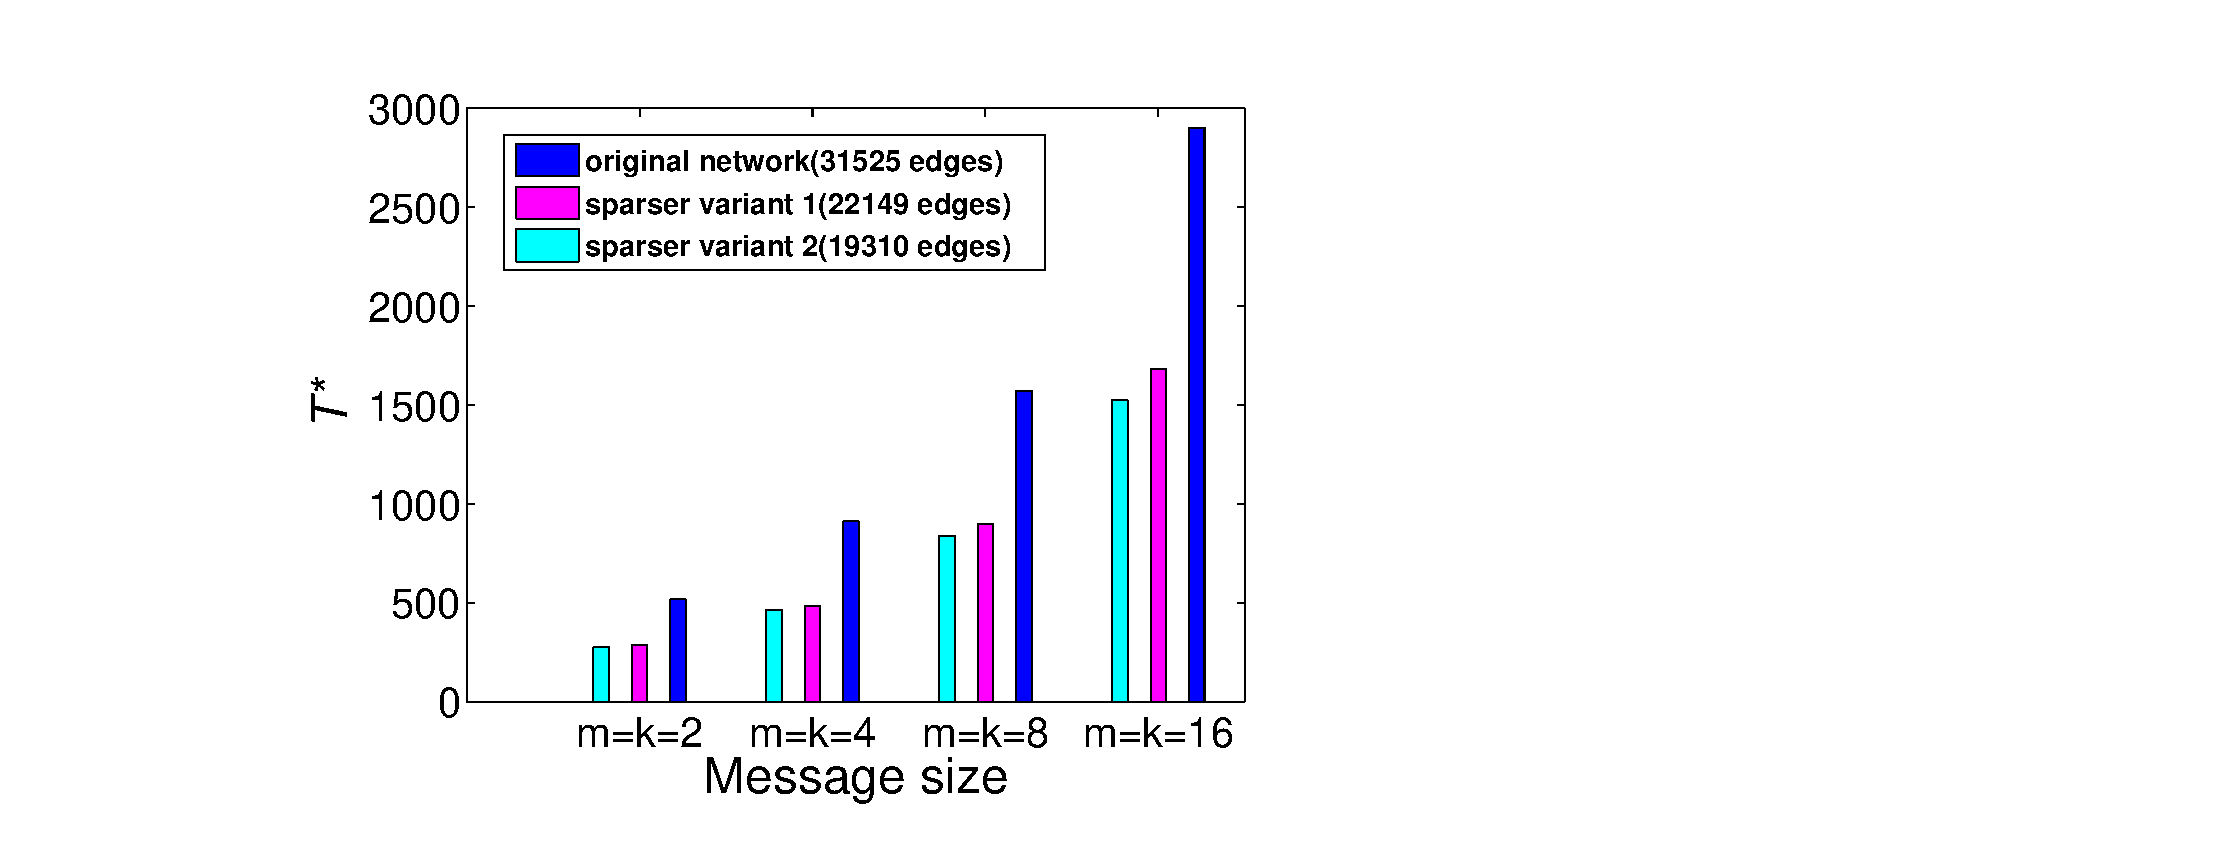
\includegraphics[scale=0.25]{figs1/gnutella2.eps}
% \caption{Broadcast time for the gnutella snapshots and their sparser variants versus different values of message sizes for gnutella1 and gnutella2\vspace{-3mm}}
% \label{gnutellasparse}
% \end{figure}
% \medskip

%\vspace{-2.5mm}
\noindent
%\vspace{-8mm}
\subsection{Comparison of different broadcast strategies on gnutella Topology}
%\vspace{-4mm}
% We measure 
% the performance of the four algorithms (B-P, X-P-P, P-G and P-P-G) on three real network traces based on broadcast time, 
% wastage and coverage. The data sets are Gnutella network snapshots namely 
% p2p-Gnutella04 (gnutella1), p2p-Gnutella06 (gnutella2) and p2p-Gnutella25 (gnutella3) ~\cite{leskovec2007graph,ripeanu2002mapping} taken on dates August 4, August 6 and August 25, 2002 respectively. 
% The gnutella1 network has 10876 nodes and 39994 edges in its largest connected component. Corresponding number of nodes and edges in the largest connected component 
% in gnutella2 and gnutella3 are respectively 8717, 31525 and 22663, 54693. We simulate these algorithms for varying message sizes.
% We perform our simulations on peer-to-peer systems specifically as our study can find a major application in such systems.

% For simulating the X-P-P algorithm in particular we first need to obtain the best value of x for each network and then run the simulations for varying message sizes. 
%  In figure ~\ref{ps_bt} and ~\ref{ps_wa}, we show how the broadcast time and wastage varies with x for gnutella1 network. We observe that the best value of x lies around 
%  50\%. Similarly we obtained the value of x for the other two datasets as well and found it to be around 50\% and 60\% for gnutella2 and gnutella3 
%  respectively.
% \begin{figure}
% \centering
% \includegraphics[scale=0.15]{figs1/xperbt.eps}
% \includegraphics[scale=0.15]{figs1/xperwa.eps}
% \caption{Average broadcast time and wastage versus x for gnutella1,gnutella2 and gnutella3\vspace{-5mm}}
% \label{ps_bt}
% \end{figure}

% \begin{figure}[htpb]
% \centering
% \includegraphics[scale=0.15]{figs1/xperwa.eps}
% \caption{average wastage time versus x for gnutella1\vspace{-5mm}}
% \label{ps_wa}
% \end{figure}
% \begin{figure*}[!ht]
%   \centering
%   \includegraphics*[width=0.65\textwidth,height=40mm,angle=0]{figs1/gnutella4_bt_wa_co.eps}
% 
%  \vspace{-5mm}
%  %\caption{\label{gnutellacomp} (A) broadcast time versus message size (B) wastage versus message size (C) coverage versus message size for gnutella1, gnutella2 and gnutella3}
% \end{figure*}
% \begin{figure*}[!ht]
%   \centering
%  \includegraphics*[width=0.65\textwidth,height=40mm,angle=0]{figs1/gnutella6_bt_wa_co.eps}	
%  \vspace{-5mm}
% 
%  
%  %\caption{\label{gnutellacomp} (A) broadcast time versus message size (B) wastage versus message size (C) coverage versus message size for gnutella1, gnutella2 and gnutella3}
% \end{figure*}
% \begin{figure}
% \centering
% \includegraphics[scale=0.15]{figs1/xperbt.eps}
% \includegraphics[scale=0.15]{figs1/xperwa.eps}
% \caption{Average broadcast time and wastage versus x for gnutella1,gnutella2 and gnutella3\vspace{-5mm}}
% \label{ps_bt}
% \end{figure}
%\medskip

\begin{figure}
\centering
\includegraphics[scale=0.19]{./texfiles/Chapter_3/netsci/figs1/random_graphs_delay1.eps}
\includegraphics[scale=0.18]{./texfiles/Chapter_3/netsci/figs1/random_graphs_wastage1.eps}
\caption{(A) Broadcast time and (B) broadcast wastage versus average degree for B-P. The parameters values are $n=200, m=4, k=2$.\vspace{4mm}}
\label{DiffTopologyGnp_N200_varyD_push_pull}
\end{figure}
\begin{figure}
\centering
\includegraphics[scale=0.19]{./texfiles/Chapter_3/netsci/figs1/xperbt.eps}
\includegraphics[scale=0.19]{./texfiles/Chapter_3/netsci/figs1/xperwa.eps}
\caption{Average broadcast time and wastage versus $x$ for gnutella1, gnutella2 and gnutella3}
\label{ps_bt}
\end{figure}


\begin{figure*}[!ht]
  \centering	
 \includegraphics*[width=0.65\textwidth,height=40mm,angle=0]{./texfiles/Chapter_3/netsci/figs1/gnutella25_bt_wa_co.eps}
%\vspace{-5mm}
 
 \caption{\label{gnutellacomp} (A) Broadcast time versus message size (B) Wastage versus message size (C) Coverage versus message size for gnutella3}
\end{figure*}


\begin{figure*}[!ht]
  \centering	
 \includegraphics*[width=0.45\textwidth,height=40mm,angle=0]{./texfiles/Chapter_3/netsci/figs1/comp_gnut_4.eps}
 \includegraphics*[width=0.45\textwidth,height=40mm,angle=0]{./texfiles/Chapter_3/netsci/figs1/comp_gnut_6.eps}
%\vspace{-5mm}
 
 \caption{\label{gnutellacomp1} Gain in broadcast time of P-P-G over X-P-P and B-P [Inset shows gain in wastage] for (A) gnutella1 and (B) gnutella2 networks. Note: algo = B-P/X-P-P }
\vspace{.5cm}
 \end{figure*}
% \begin{figure*}[!ht]
%   \centering	
%  \includegraphics*[width=0.65\textwidth,height=40mm,angle=0]{figs1/gnutella25_bt_wa_co.eps}
% \vspace{-5mm}
%  
%  \caption{\label{gnutellacomp} (A) Broadcast time versus message size (B) Wastage versus message size (C) Coverage versus message size for gnutella1, gnutella2 and gnutella3\vspace{-3mm}}
% \end{figure*}

We measure 
the performance of the algorithms (B-P, X-P-P and P-P-G) on three real network traces based on broadcast time, 
wastage and coverage. The data sets are Gnutella network snapshots namely 
p2p-Gnutella04 (gnutella1), p2p-Gnutella06 (gnutella2) and p2p-Gnutella25 (gnutella3)~\cite{leskovec2007graph,ripeanu2002mapping} taken on dates August 4, August 6 and August 25, 2002 respectively. 
The gnutella1 network has 10876 nodes and 39994 edges in its largest connected component. Corresponding number of nodes and edges in the largest connected component 
in gnutella2 and gnutella3 are respectively 8717, 31525 and 22663, 54693. We simulate these algorithms for varying message sizes.
We perform our simulations on peer-to-peer systems specifically as our study can find a major application in such systems.

For simulating the X-P-P algorithm in particular we first need to obtain the best value of $x$ for each network and then run the simulations for varying message sizes. 
 In figure~\ref{ps_bt}, we show how the broadcast time and wastage varies with $x$ for networks gnutella1, gnutella2 and gnutella3. We observe that the best value of $x$ lies around 
 50\% for the gnutella1 network. Similarly the obtained value of $x$ are found to be around 50\% and 60\% for gnutella2 and gnutella3 
 respectively.
% We measure the performance of the three algorithms (B-P, P-G and P-P-G) on three real network traces based on broadcast time, 
% wastage and coverage. The data sets are Gnutella snapshots namely 
% p2p-Gnutella04 (gnutella1), p2p-Gnutella06 (gnutella2) and p2p-Gnutella25 ~\cite{ripeanu2002mapping,leskovec2007graph} taken on dates August 4, August 6 and August 25, 2002 respectively. 
% The gnutella1 network has 10876 nodes and 39994 edges in its largest connected component. Corresponding number of nodes and edges in the largest connected component 
% in gnutella2 and gnutella3 are respectively 8717, 31525 and 22663, 54693. We simulate these algorithms for varying message sizes.
% 
% For simulating the X-P-P algorithm we first obtain the best value of x for each network and then run the simulations for varying message sizes. 
%  In figure ~\ref{ss} and ~\ref{}, we show how the broadcast time and wastage varies with x for gnutella1 network. We obsreve that the best value of x lies around 
%  50\%. Similarly we obtained the value of x for the other two datasets as well and found it to be around 50\% and 60\% for gnutella2 and gnutella3 
%  respectively.
% As mentioned earlier we observe from simulation results (shown in figure [4]) that the P-G algorithm performs better than B-P with respect to broadcast time and 
%  wastage with a reasonably good coverage of around 95\% when message size is 2. However, the coverage drastically falls as we increase the message size. 
%  P-P-G performs best among all the algorithms in terms of broadcast time.
%  It is so because the non-sender nodes are allowed $pull$ opportunities in addition to $push$ by 
%  sender nodes. In addition, it can be noticed that the overall wastage with respect to B-P is also reduced significantly. 
%  X-P-P performs best in terms of wastage and is second only to P-P-G in terms of broadcast time. Actually, X-P-P provides the best optimization 
%   between broadcast time and wastage but would incur significant computational overhead if implemented; in fact, it is infeasible in practical distributed settings.
%  Note that it is almost impossible to have an algorithm which optimizes both broadcast time and wastage yet providing maximum coverage.
%  Our proposed algorithm (P-P-G) presents the best possible trade-off of delay and wastage guaranteeing almost 100\% coverage and can be 
%  implemented in a distributed fashion with almost negligible computational overhead.
In figure ~\ref{gnutellacomp} we plot the broadcast time, wastage and coverage for gnutella3 network. 
We observe that with P-P-G we gain in both broadcast time and wastage with respect to B-P. With respect to X-P-P, P-P-G offers better 
broadcast time but with a higher wastage.
For gnutella1 and gnutella2 networks 
we plot (figure ~\ref{gnutellacomp1}) the ratio of broadcast time and wastage of X-P-P and B-P over P-P-G for different message sizes. 
% We observe that accross different message sizes on an average the ratio of broadcast time of X-P-P over P-P-G is around $1.5$ and that for B-P over P-P-G is $5.8$. 
% The corresponding values for wastage are $0.75$ and $1.10$ respectively. 
We observe that across different message sizes, on average the increase in broadcast time of X-P-P over P-P-G and B-P over P-P-G are $5.45$ and $1.5$ respectively for 
gnutella1 network while for gnutella2 network the corresponding values are 5.9 and 1.6 respectively. Corresponding values for wastage are $0.75$ and $1.10$ 
respectively for gnutella1 network and $0.72$ and $1.06$ respectively for gnutella2 network. 
So with P-P-G we gain in both broadcast time and wastage with respect to B-P while with respect to X-P-P 
we gain in broadcast time without significant increase in wastage.
 Actually, X-P-P provides the best optimization between broadcast time and wastage but it would be hard to implement in a 
distributed setting. 
Our proposed algorithm (P-P-G) presents the best possible trade-off between delay and wastage guaranteeing almost 100\% coverage and can be implemented in a distributed fashion with almost negligible computational overhead.
% \begin{figure*}[!ht]
%   \centering
%   \includegraphics*[width=0.65\textwidth,height=40mm,angle=0]{figs1/gnutella4_bt_wa_co.eps}
% 
%  \vspace{-5mm}
%  %\caption{\label{gnutellacomp} (A) broadcast time versus message size (B) wastage versus message size (C) coverage versus message size for gnutella1, gnutella2 and gnutella3}
% \end{figure*}
% \begin{figure*}[!ht]
%   \centering
%  \includegraphics*[width=0.65\textwidth,height=40mm,angle=0]{figs1/gnutella6_bt_wa_co.eps}	
%  \vspace{-5mm}
% 
%  
%  %\caption{\label{gnutellacomp} (A) broadcast time versus message size (B) wastage versus message size (C) coverage versus message size for gnutella1, gnutella2 and gnutella3}
% \end{figure*}
% 
% \begin{figure*}[!ht]
%   \centering	
%  \includegraphics*[width=0.45\textwidth,height=40mm,angle=0]{figs1/comp_gnut_4.eps}
%  \includegraphics*[width=0.45\textwidth,height=40mm,angle=0]{figs1/comp_gnut_6.eps}
% \vspace{-5mm}
%  
%  \caption{\label{gnutellacomp1} Efficiency in broadcast time of P-P-G over X-P-P and B-P for gnutella1 and gnutella2 networks. (inset) efficiency in wastage of P-P-G over X-P-P and P-G \vspace{-10mm}}
% \end{figure*}
% We measure the performance of the three algorithms (B-P, P-G and P-P-G) on three real network traces based on broadcast time, 
% wastage and coverage. The data sets are Gnutella snapshots namely 
% p2p-Gnutella04 (gnutella1), p2p-Gnutella06 (gnutella2) and p2p-Gnutella25 ~\cite{ripeanu2002mapping,leskovec2007graph} taken on dates August 4, August 6 and August 25, 2002 respectively. 
% The gnutella1 network has 10876 nodes and 39994 edges in its largest connected component. Corresponding number of nodes and edges in the largest connected component 
% in gnutella2 and gnutella3 are respectively 8717, 31525 and 22663, 54693. We simulate these algorithms for varying message sizes.

% \begin{figure*}[!ht]
%   \centering
%   \includegraphics*[width=0.7\textwidth,height=55mm,angle=0]{figs1/gnutella4_bt_wa_co.eps}
% 
%  \vspace{-5mm}
%  %\caption{\label{gnutellacomp} (A) broadcast time versus message size (B) wastage versus message size (C) coverage versus message size for gnutella1, gnutella2 and gnutella3}
% \end{figure*}
% \begin{figure*}[!ht]
%   \centering
%  \includegraphics*[width=0.7\textwidth,height=55mm,angle=0]{figs1/gnutella6_bt_wa_co.eps}	
%  \vspace{-5mm}
% 
%  
%  %\caption{\label{gnutellacomp} (A) broadcast time versus message size (B) wastage versus message size (C) coverage versus message size for gnutella1, gnutella2 and gnutella3}
% \end{figure*}
% \begin{figure*}[!ht]
%   \centering	
%  \includegraphics*[width=0.7\textwidth,height=55mm,angle=0]{figs1/gnutella25_bt_wa_co.eps}
% \vspace{-5mm}
%  
%  \caption{\label{gnutellacomp} (A) broadcast time versus message size (B) wastage versus message size (C) coverage versus message size for gnutella1, gnutella2 and gnutella3}
% \end{figure*}
%  \begin{figure}
% \centering
% 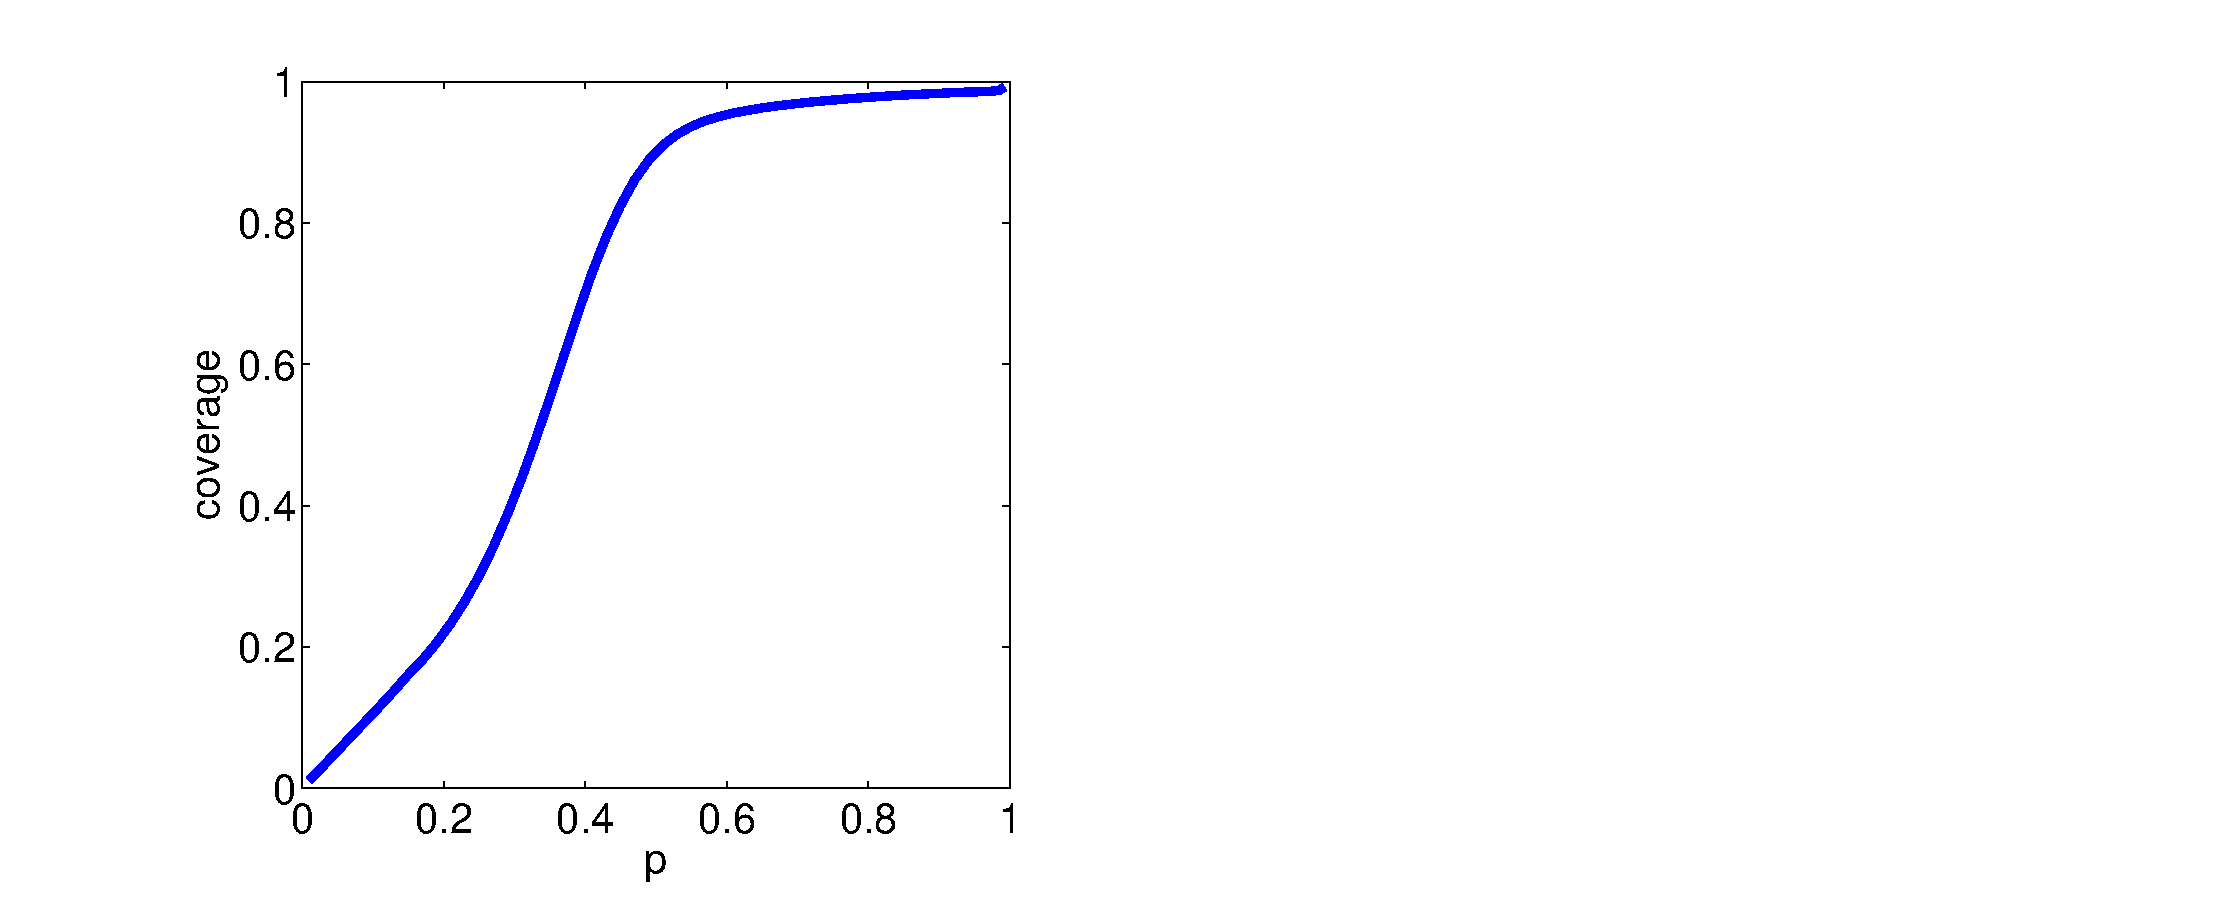
\includegraphics[scale=0.4]{figs1/pvsco.eps}
% \caption{(A) Broadcast time and (B) broadcast wastage versus different values of $d$ for B-P. The parameters values are $n=200, m=4, k=2$.\vspace{-3mm}}
% \label{pcov}
% \end{figure}
%  For simulating the X-P-P algorithm we first obtain the best value of x for each network and then run the simulations for varying message sizes. 
%  In figure ~\ref{ss} and ~\ref{}, we show how the broadcast time and wastage varies with x for gnutella1 network. We obsreve that the best value of x lies around 
%  50\%. Similarly we obtained the value of x for the other two datasets as well and found it to be around 50\% and 60\% for gnutella2 and gnutella3 
%  respectively.
 
%  As mentioned earlier we observe from simulation results (shown in figure [4]) that the P-G algorithm performs better than B-P with respect to broadcast time and 
%  wastage with a reasonably good coverage of around 95\% when message size is 2. However, the coverage drastically falls as we increase the message size. 
%  P-P-G performs best among all the algorithms in terms of broadcast time.
%  It is so because the non-sender nodes are allowed $pull$ opportunities in addition to $push$ by 
%  sender nodes. In addition, it can be noticed that the overall wastage with respect to B-P is also reduced significantly. 
%  X-P-P performs best in terms of wastage and is second only to P-P-G in terms of broadcast time. Actually, X-P-P provides the best optimization 
%   between broadcast time and wastage but would incur significant computational overhead if implemented; in fact, it is infeasible in practical distributed settings.
%  Note that it is almost impossible to have an algorithm which optimizes both broadcast time and wastage yet providing maximum coverage.
%  Our proposed algorithm (P-P-G) presents the best possible trade-off of delay and wastage guaranteeing almost 100\% coverage and can be 
%  implemented in a distributed fashion with almost negligible computational overhead.
%  We also mentioned previously that the condition for give-up has a factor $p$ 
%  (we consider the threshold for give-up to be $f*(|l_{i}|+1)$ and $f=-\log(1-p)$) through which we can control the coverage. 
%  In figure [5] we plot the value of $p$ versus coverage for gnutella1 network. We observe that the coverage increases gradually as we 
%  increase $p$. So, for a greater coverage one needs to use a sufficiently large value of $p$ and vice-versa. 
%  We show this effect only empirically in this 
%  paper but we plan to analyze it in more details analytically in a forthcoming paper.
% \begin{figure}
% \centering
% 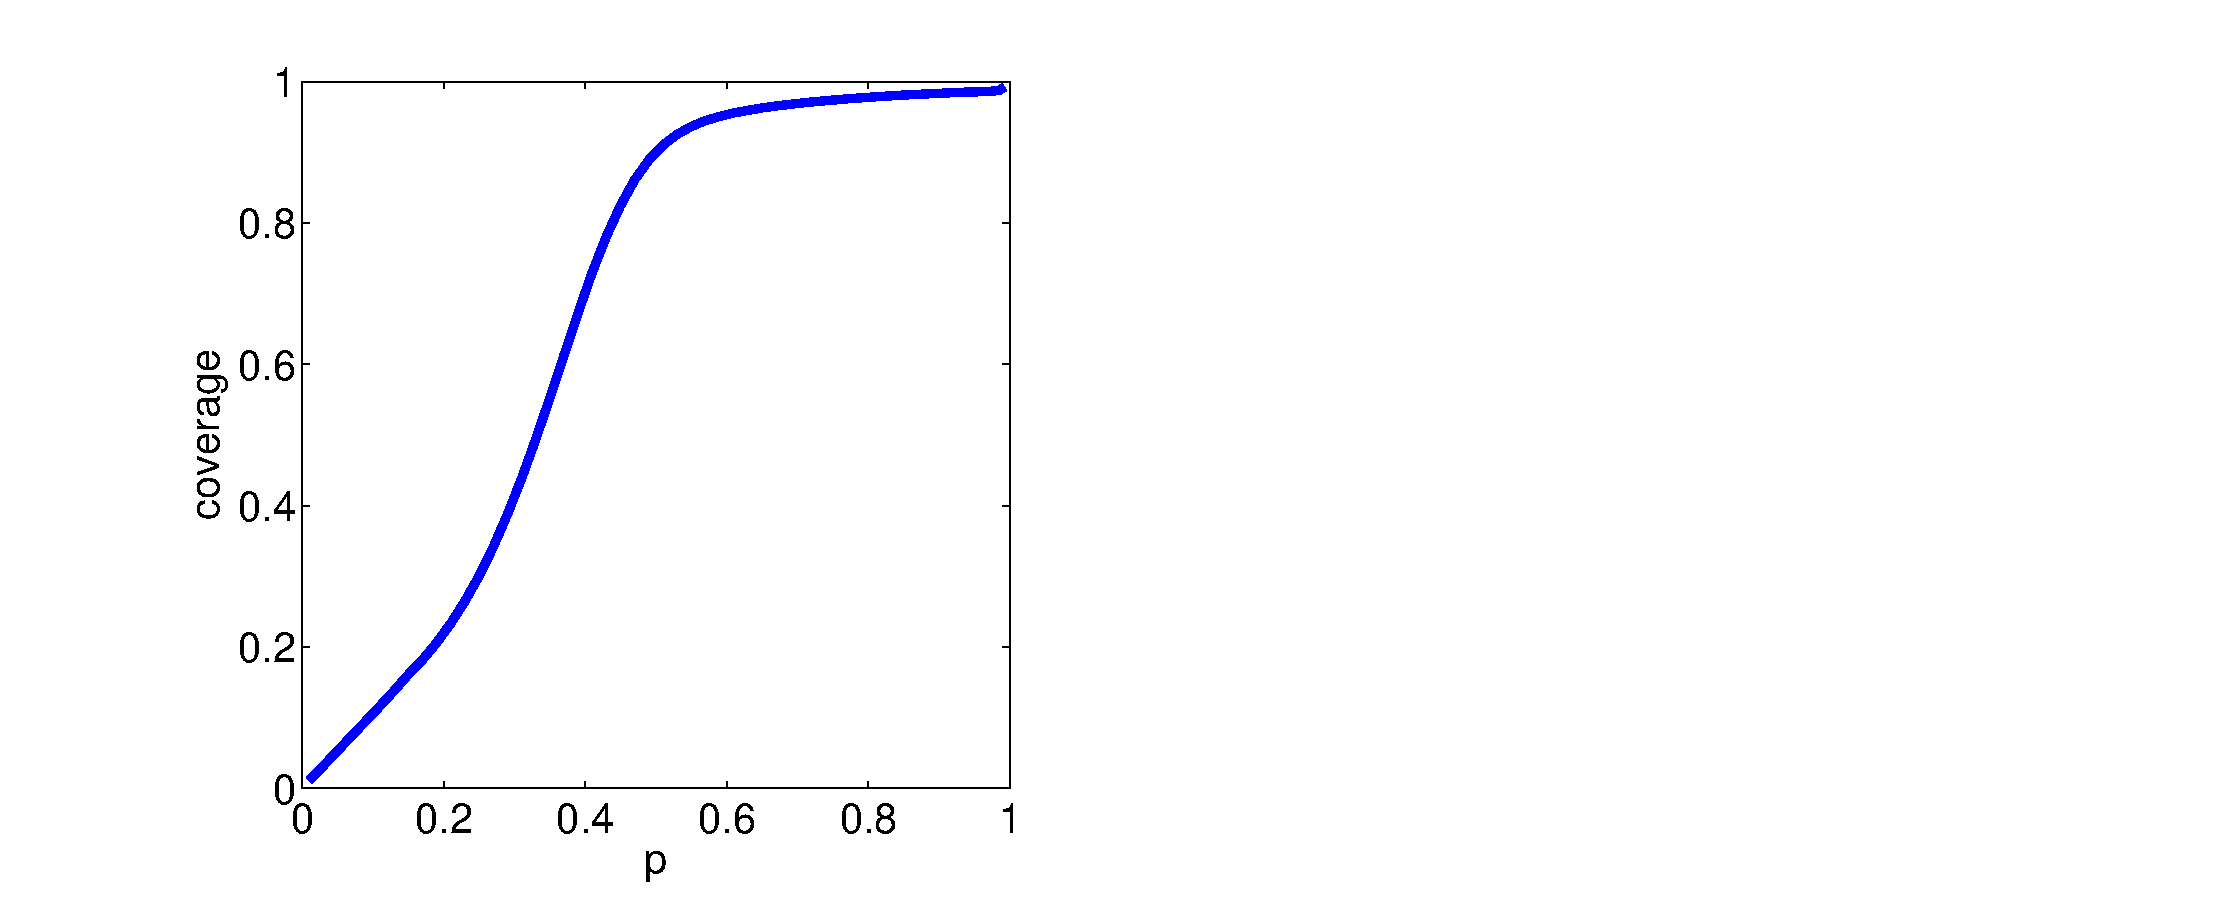
\includegraphics[scale=0.4]{figs1/pvsco.eps}
% \caption{$p$ versus coverage for gnutella1 network\vspace{-3mm}}
% \label{pcov}
% \end{figure}
%\vspace{-2mm}
\subsubsection{Effect of degree on broadcast time}

  In earlier part of this section we observed that irrespective of the topology one is able to  
obtain a critical value of $d$ for which the 
  broadcast time is minimum. So we perform simulations on sparser variants of these gnutella networks
and observe that broadcast time reduces even for the B-P. To obtain sparser variants, we consider each gnutella snapshot and randomly removed 
some of the edges 
without hampering the network connectivity. From figure ~\ref{gnutellasparse} we observe that the broadcast time reduces significantly
in case of the sparser variants in comparison to the original network.
Hence, while designing a network it is advisable to keep the network sparse rather than creating unnecessary connections between the nodes.
This, as our results indicate, should lead to a faster dissemination of messages.


% Since the value of the critical average degree is found to be on the lower side, we performed simulations on sparser variants of the real traces (used previously)
% and observed that broadcast time reduces even for the B-P. We considered each gnutella snapshot and randomly removed some of the edges such that the
% network remains connected while producing a sparser variant. From figure ~\ref{gnutellasparse} we observe that the broadcast time reduces significantly
% in case of the sparser variants in comparison to the original network.
% Hence, while designing a network it is advisable to keep the network sparse rather than creating unnecessary connections between the nodes.
% This, as our results indicate, should lead to a faster dissemination of messages.

\begin{figure}
\centering
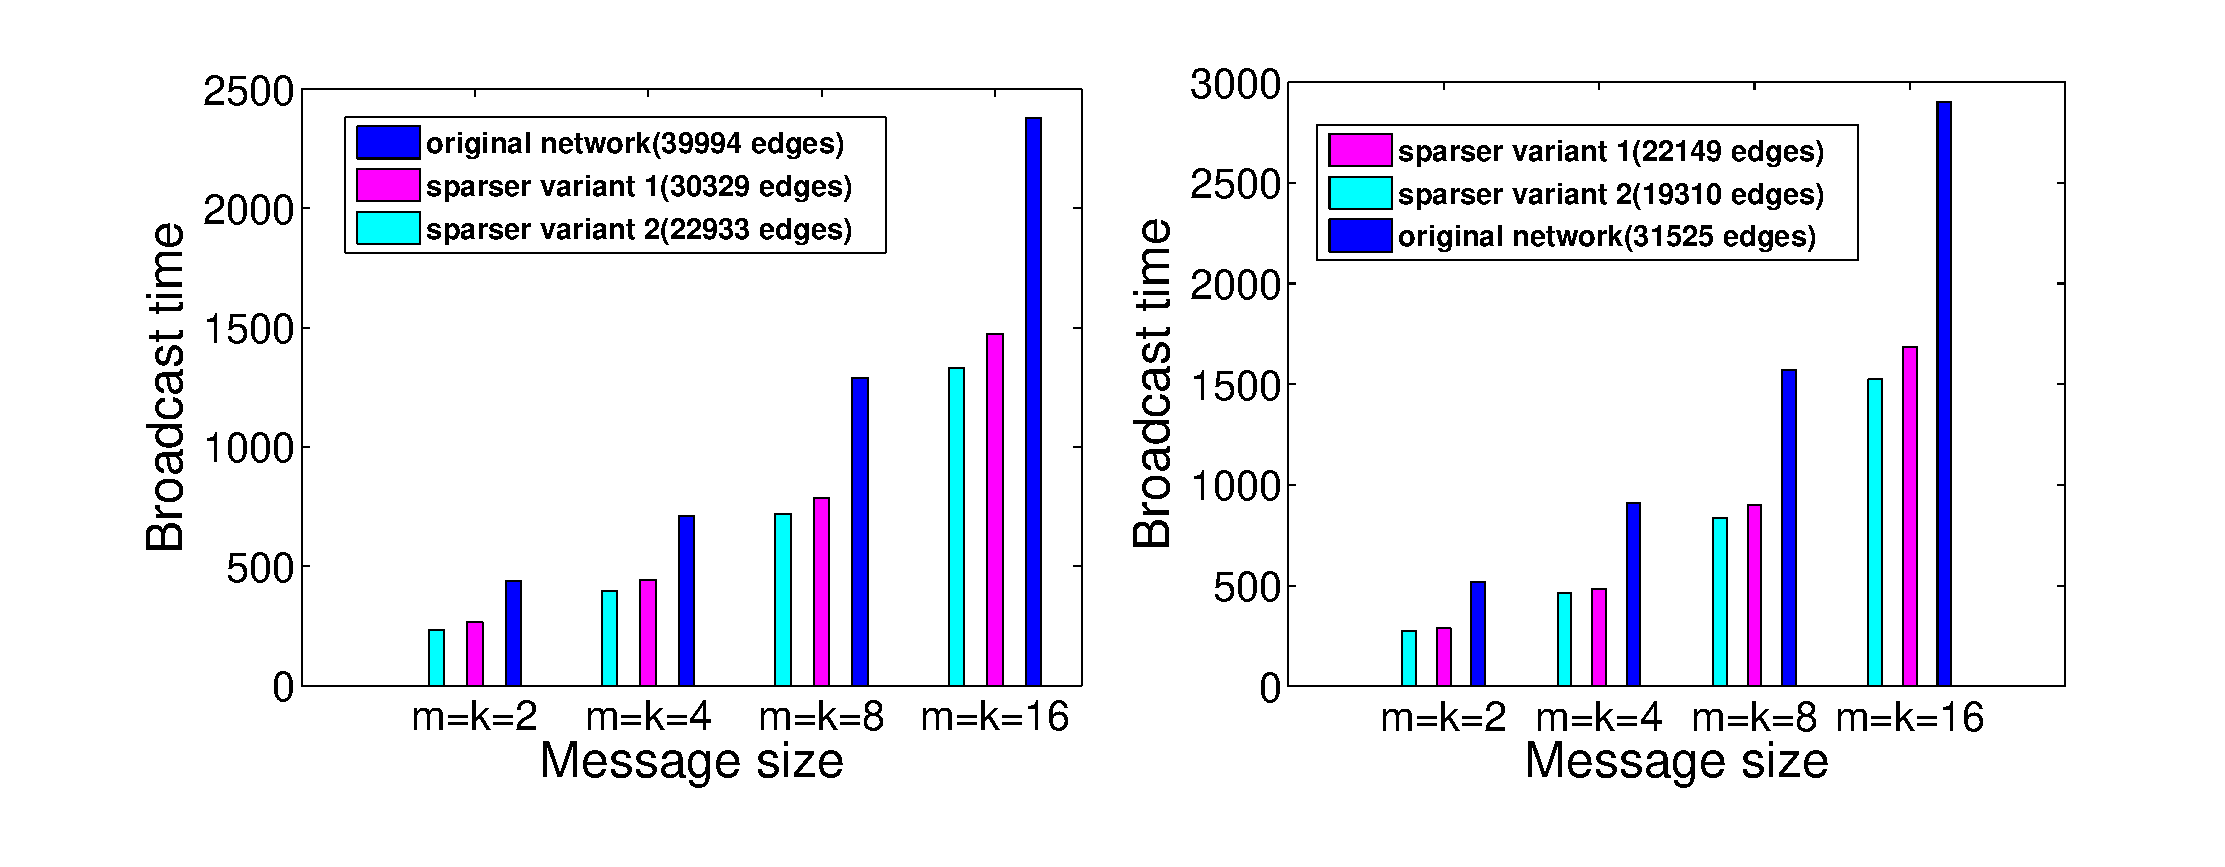
\includegraphics[scale=0.25]{./texfiles/Chapter_3/netsci/figs1/gnutella1_gnutella2.eps}
%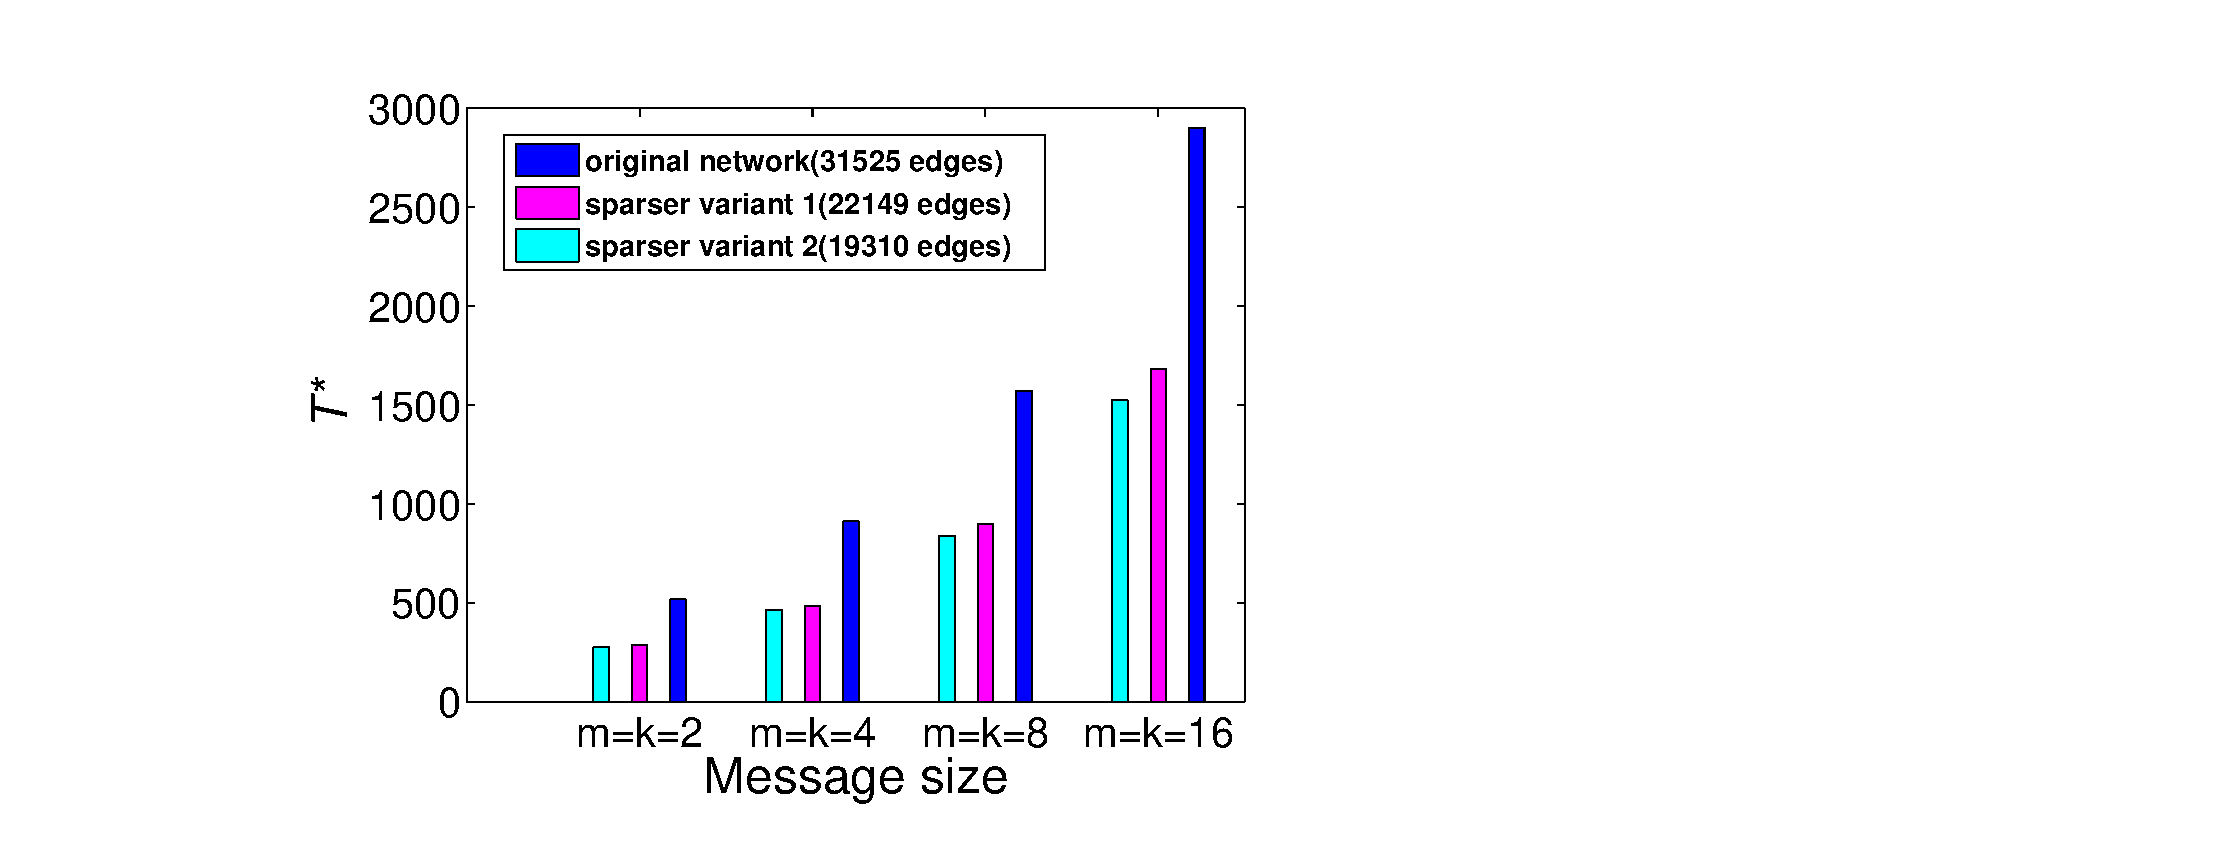
\includegraphics[scale=0.25]{figs1/gnutella2.eps}
%\vspace{-8mm}
\caption{Broadcast time for the gnutella snapshots and their sparser variants versus different values of message sizes for (a). gnutella1 and (b). gnutella2}
\label{gnutellasparse}
\vspace{.5cm}
\end{figure}
\medskip

 \medskip

%\vspace{-7mm}
% \section{Theoretical analysis}
% \label{theory}
% \noindent
In this section, we first show through numerical simulations that the time to create the first sender, i.e., $T_1$, almost fully determines the overall broadcast time $T^*$. Next, we present an analytical treatment of the push technique for the minimum non-trivial case of $m=k=2$. In particular,  we attempt to compute the expected value of $T_1$ (i.e., $E(T_1)$) which is also supposed to provide an approximate estimation of $E(T^*)$. Finally, we provide pointers for the analytical treatment of the general $m=k$ case.  
We concentrate particularly on the complete graph topology; however, in a later subsection we also analytically study the message propagation for  
$m=k$ on infinite regular trees
\vspace{-3mm}
\subsection{Numerical simulations on complete graph topology}
\vspace{-1mm}



In this section, we give numeric evidence (with analytical support) that the
ratio of the overall broadcast time $T^{\ast }$ and the time to
create the first sender, i.e., $T_{1}$ converges for $n\rightarrow \infty$ to a constant which only depends on $k$. For this purpose we plot in figure~\ref%
{segSizeVsDelay_nrTrans_varyN_Mall_push_pull} the values of $Av(T^{\ast })$
and $Av(T_{1})$ respectively as we vary $n$ where $Av(x)$ represents the average of the quantity $x$ over several simulation runs. We report this distribution for
four different values of $m$ (2, 4, 8 and 16), in each case assuming that
there is only one message segment, i.e., $k=m$. Note that for B-P, the two quantities $Av(T^{\ast })$ and $Av(T_{1})$
exhibit a very similar profile irrespective of the value of $m$ chosen. In the same figure we also plot the function $n^{\frac{k-1}{k}}$ suitably scaled by a constant to show how the theoretical results which we provide in the following sections, closely approximate the numerical simulations. 

\begin{figure}[htbp] 
\centering
\includegraphics[scale=0.36]{figs1/segSizeVsDelay_nrTrans_varyN_Mall_push_pull2.eps}
\caption{$Av(T^*)$ and $Av(T_1)$ versus the number of nodes ($n$). Results are presented for (A) $m=k=2$, (B) $m=k=4$, (C) $m=k=8$, and (D) $m=k=16$. The plots also contain the suitably scaled function $n^{\frac{k-1}{k}}$ for each case.}
\label{segSizeVsDelay_nrTrans_varyN_Mall_push_pull}
\end{figure}
\vspace{-3mm}
\subsection{Performance of B-P in the limit $n\rightarrow \infty$ for complete graph topology}
\vspace{-1mm}


% We compute the expected time to obtain the first sender $E(T_{1})$ as well
% as the expected time $E\left( T^{\ast }\right) $ for broadcasting for a
% message which has $m=2$ packets ($p_{1}$ and $p_{2}$), and $s=1$ segment
% (i.e., the segment has $k=2$ packets). Recall that in push epidemic
% protocol, in each time step, a sender tries to establish a communication
% link with another agent. 
% %In each contact opportunity, only one packet can be
% %transferred from a sender to a receiver.
% As mentioned earlier, we assume only one packet can be transferred from a sender to a receiver in each contact opportunity. 
% 
% At the beginning, a source agent creates a message having 2 packets at time $%
% T_{0}$, this message has to be delivered to all other agents (i.e., $n-1$
% agents) in the network. The number of senders as a function of time is a
% step function and we denote the time of the $i^\textrm{th}$ step by $t_{i}.$ For $i$
% not too large  $\sum\limits_{j=1}^{i}t_{j}$ gives essentially the time $T_{i}$
% when the $i^\textrm{th}$ sender will be created, with the convention that $T_{0}=0$.
% Note that $\sum\limits_{i\geq 1}t_{i}$ is the broadcast time $T^{\ast }$ and 
% $t_{1}$ is the time when the first new sender is created.
% \vspace{-2mm}
% \begin{theorem}
% The random variable $\frac{t_{1}}{\sqrt{n}}$ converges as $n\rightarrow \infty $ to a
% limiting random variable $\tau _{1}$ with density $xe^{-\frac{x^{2}}{2}}$ and
% expectation $E\left( \tau _{1}\right) =\sqrt{\frac{\pi }{2}}.$ Furthermore
% for fixed $i\geq 2$ the random variable $\frac{t_{i}}{\sqrt{n}}$ converges to a
% limiting random variable $\tau _{i}$ and the following recursion holds for the
% expectations: $\frac{E\left( \tau _{i}\right) }{E\left( \tau _{i-1}\right) }%
% =\left( 1-\frac{3}{2i}\right) .$
% \end{theorem}
% \vspace{-2mm}
% \begin{theorem}
% $\frac{T^{\ast }}{\sqrt{n}}$ converges to a limiting random variable $s^{\ast }$ with $%
% E\left( s^{\ast }\right) =\sum\limits_{i=1}^{\infty }E\left( \tau
% _{i}\right) =2\cdot \sqrt{\frac{\pi }{2}}$
% \end{theorem}
% \vspace{-3mm}
% \begin{proof}
% (sketch). We will sketch in the following some of the important steps in the
% proof. For the probability that the first new sender is created at time $t$
% we have%
% \[
% \Pr \left\{ t_{1}=t\right\} =\frac{t-1}{n}\prod\limits_{l=1}^{t-2}\left( 1-%
% \frac{l}{n}\right) ,t\geq 2
% \]%
% Writing $\left( 1-\frac{l}{n}\right) =e^{-\frac{l}{n}+O\left( \frac{l^{2}}{%
% n^{2}}\right) }$we have for the cumulative distribution function 
% \begin{eqnarray*}
% \Pr \left\{ \frac{t_{1}}{\sqrt{n}}\leq x\right\}  &=&\sum\limits_{t\leq x%
% \sqrt{n}}\frac{t-1}{n}\prod\limits_{l=1}^{t-2}\left( 1-\frac{l}{n}\right)  \\
% &=&\sum\limits_{t\leq x\sqrt{n}}\frac{t}{n}e^{-\frac{t^{2}}{2n}+O\left( 
% \frac{t^{3}}{n^{2}}\right) }
% \end{eqnarray*}%
% For $n\rightarrow \infty $, the sum in the last expression converges to $%
% \int\limits_{0}^{x}ye^{-\frac{y^{2}}{2}}dy.$  Hence the limiting density is
% given by $ye^{-\frac{y^{2}}{2}}$ and the expectation by $\int\limits_{0}^{%
% \infty }y^{2}e^{-\frac{y^{2}}{2}}dy=\sqrt{\frac{\pi }{2}}.$ In a similar
% fashion one can obtain the conditional limiting distribution of $\tau _{i}$
% given the value of $b_{i-1}:=\sum\limits_{m=1}^{i-1}m\tau _{m}:$ 
% \[
% \Pr \left\{ \tau _{i}\leq x\right\} =\int\limits_{0}^{x}i\left(
% b_{i-1}+i\tau _{i}\right) e^{-i\left( \tau _{i}b_{i-1}+k\tau
% _{i}^{2}/2\right) }d\tau _{i}
% \]%
% Note that $b_{i}\sqrt{n}$ is the approximate number of nodes with one
% packet up to time $T_{i}.$ By a straightforward but lengthy computation
% using the previous expression for the conditional distribution of $\tau _{i}$
% it can be shown that the recursion $\frac{E\left( \tau _{i}\right) }{E\left(
% \tau _{i-1}\right) }=\left( 1-\frac{3}{2i}\right) $ holds. We will derive
% from this recursion now the expression for $s^{\ast }.$ Clearly we have 
% \[
% E\left( \tau _{i}\right) =\prod\limits_{j\geq 2}^{i}\frac{2j-3}{2j}E\left(
% \tau _{1}\right) 
% \]%
% and hence $s^{\ast }=\left( 1+\sum\limits_{i\geq 2}\prod\limits_{j\geq 2}^{i}%
% \frac{2j-3}{2j}\right) E\left( \tau _{1}\right) .$ Rewriting the product as%
% \[
% \prod\limits_{j\geq 2}^{i}\frac{2j-3}{2j}=\frac{\left( 2\left( i-1\right)
% \right) !}{4^{i-1}\left( \left( i-1\right) !\right) ^{2}i}
% \]%
% we have%
% \[
% s^{\ast }=\left( \sum\limits_{i=0}\frac{\left( 2i\right) !\cdot 2}{%
% 4^{i-1}\left( i!\right) ^{2}\cdot 2\left( i+1\right) }\right) E\left( \tau
% _{1}\right) 
% \]%
% The function 
% \[
% g\left( z\right) :=\sum\limits_{i=0}\frac{\left( 2i\right) !}{%
% 4^{i-1}\left( i!\right) ^{2}\cdot 2\left( i+1\right) }z^{2\left( i+1\right) }
% \]%
% converges for $\left\vert z\right\vert \leq 1$ and satisfies%
% \[
% \frac{d}{dz}g\left( z\right) =z\cdot \frac{d}{dz}\arcsin z=z\cdot \frac{1}{%
% \sqrt{1-z^{2}}}
% \]%
% as can be easily seen by comparing with the Taylor expansion of the right hand side. Hence 
% \[
% g\left( 1\right) =\int\limits_{0}^{1}\frac{z}{\sqrt{1-z^{2}}}dz=1
% \]%
% and $s^{\ast }=2E\left( \tau _{1}\right).$
% \end{proof}
% 
% It is important to note that the above computations can be carried out essentially up to a time $t$ where there are $\sqrt{n}$ senders. The remaining growth is very fast - actually of logarithmic order since several new senders in every time step get produced.
% \vspace{-3mm}
We compute the expected time to obtain the first sender $E(T_{1})$ as well
as the expected time $E\left( T^{\ast }\right) $ for broadcasting for a
message which has $m=2$ packets ($p_{1}$ and $p_{2}$), and $s=1$ segment
(i.e., the segment has $k=2$ packets). Recall that in push epidemic
protocol, in each time step, a sender tries to establish a communication
link with another agent. 
%In each contact opportunity, only one packet can be
%transferred from a sender to a receiver.
As mentioned earlier, we assume only one packet can be transferred from a
sender to a receiver in each contact opportunity.

At the beginning, a source agent creates a message having 2 packets at time $%
T_{0}$, this message has to be delivered to all other agents (i.e., $n-1$
agents) in the network. The number of senders as a function of time is a
step function and we denote the time of the $i^\textrm{th}$ step by $t_{i}.$
For $i$ not too large $\sum\limits_{j=1}^{i}t_{j}$ gives essentially the
time $T_{i}$ when the $i^\textrm{th}$ sender will be created, with the
convention that $T_{0}=0$. Note that $\sum\limits_{i\geq 1}t_{i}$ is the
broadcast time $T^{\ast }$ and $t_{1}$ is the time when the first new sender
is created. \vspace{-2mm} 
\begin{theorem}
The random variable $\frac{t_{1}}{\sqrt{n}}$ converges as $n\rightarrow \infty $ to a
limiting random variable $\tau _{1}$ with density $xe^{-\frac{x^{2}}{2}}$ and
expectation $E\left( \tau _{1}\right) =\sqrt{\frac{\pi }{2}}.$ Furthermore
for fixed $i\geq 2$ the random variable $\frac{t_{i}}{\sqrt{n}}$ converges to a
limiting random variable $\tau _{i}$ and the following recursion holds for the
expectations: $\frac{E\left( \tau _{i}\right) }{E\left( \tau _{i-1}\right) }%
=\left( 1-\frac{3}{2i}\right) .$
\end{theorem}
\vspace{-2mm} 
\begin{theorem}
$\frac{T^{\ast }}{\sqrt{n}}$ converges to a limiting random variable $s^{\ast }$ with $%
E\left( s^{\ast }\right) =\sum\limits_{i=1}^{\infty }E\left( \tau
_{i}\right) =2\cdot \sqrt{\frac{\pi }{2}}$
\end{theorem}
\vspace{-3mm} 
\begin{proof}
(sketch). We will sketch in the following some of the important steps in the
proof. For the probability that the first new sender is created at time $t$
we have%
\[
\Pr \left\{ t_{1}=t\right\} =\frac{t-1}{n}\prod\limits_{l=1}^{t-2}\left( 1-%
\frac{l}{n}\right) ,t\geq 2
\]%
Writing $\left( 1-\frac{l}{n}\right) =e^{-\frac{l}{n}+O\left( \frac{l^{2}}{%
n^{2}}\right) }$we have for the cumulative distribution function 
\begin{eqnarray*}
\Pr \left\{ \frac{t_{1}}{\sqrt{n}}\leq x\right\}  &=&\sum\limits_{t\leq x%
\sqrt{n}}\frac{t-1}{n}\prod\limits_{l=1}^{t-2}\left( 1-\frac{l}{n}\right)  \\
&=&\sum\limits_{t\leq x\sqrt{n}}\frac{t}{n}e^{-\frac{t^{2}}{2n}+O\left( 
\frac{t^{3}}{n^{2}}\right) }
\end{eqnarray*}%
For $n\rightarrow \infty $, the sum in the last expression converges to $%
\int\limits_{0}^{x}ye^{-\frac{y^{2}}{2}}dy.$  Hence the limiting density is
given by $ye^{-\frac{y^{2}}{2}}$ and the expectation by $\int\limits_{0}^{%
\infty }y^{2}e^{-\frac{y^{2}}{2}}dy=\sqrt{\frac{\pi }{2}}.$ In a similar
fashion one can obtain the conditional limiting distribution of $\tau _{i}$
given the value of $b_{i-1}:=\sum\limits_{m=1}^{i-1}m\tau _{m}:$ 
\[
\Pr \left\{ \tau _{i}\leq x\right\} =\int\limits_{0}^{x}i\left(
b_{i-1}+i\tau _{i}\right) e^{-i\left( \tau _{i}b_{i-1}+k\tau
_{i}^{2}/2\right) }d\tau _{i}
\]%
Note that $b_{i}\sqrt{n}$ is the approximate number of nodes with one
packet up to time $T_{i}.$ By a straightforward but lengthy computation
using the previous expression for the conditional distribution of $\tau _{i}$
it can be shown that the recursion $\frac{E\left( \tau _{i}\right) }{E\left(
\tau _{i-1}\right) }=\left( 1-\frac{3}{2i}\right) $ holds. We will derive
from this recursion now the expression for $s^{\ast }.$ Clearly we have 
\[
E\left( \tau _{i}\right) =\prod\limits_{j\geq 2}^{i}\frac{2j-3}{2j}E\left(
\tau _{1}\right) 
\]%
and hence $s^{\ast }=\left( 1+\sum\limits_{i\geq 2}\prod\limits_{j\geq 2}^{i}%
\frac{2j-3}{2j}\right) E\left( \tau _{1}\right) .$ Rewriting the product as%
\[
\prod\limits_{j\geq 2}^{i}\frac{2j-3}{2j}=\frac{\left( 2\left( i-1\right)
\right) !}{4^{i-1}\left( \left( i-1\right) !\right) ^{2}i}
\]%
we have%
\[
s^{\ast }=\left( \sum\limits_{i=0}\frac{\left( 2i\right) !\cdot 2}{%
4^{i-1}\left( i!\right) ^{2}\cdot 2\left( i+1\right) }\right) E\left( \tau
_{1}\right) 
\]%
The function 
\[
g\left( z\right) :=\sum\limits_{i=0}\frac{\left( 2i\right) !}{%
4^{i-1}\left( i!\right) ^{2}\cdot 2\left( i+1\right) }z^{2\left( i+1\right) }
\]%
converges for $\left\vert z\right\vert \leq 1$ and satisfies%
\[
\frac{d}{dz}g\left( z\right) =z\cdot \frac{d}{dz}\arcsin z=z\cdot \frac{1}{%
\sqrt{1-z^{2}}}
\]%
as can be easily seen by comparing with the Taylor expansion of the right hand side. Hence 
\[
g\left( 1\right) =\int\limits_{0}^{1}\frac{z}{\sqrt{1-z^{2}}}dz=1
\]%
and $s^{\ast }=2E\left( \tau _{1}\right).$
\end{proof}

It is important to note that the above computations can be carried out
essentially up to a time $t$ where there are $\sqrt{n}$ senders. The
remaining growth is very fast - actually of logarithmic order since several
new senders in every time step get produced. \vspace{-2mm}
\subsection{A short indication of the results for the general case $m=k$}
\vspace{-1mm}
% Here we present a sketch of the approach to general $m=k$ case. We are
% interested in the waiting time $t_{1}$ for the appearance of the first
% sender. For that, one has to understand how the number of sites which have
% exactly say $l$ packets grows with $t.$ 
% 
% (i) 1-packet carriers grow essentially as $t$ (because the initial sender
% node establishes contacts in most cases, a new node from the pool $n$),
% 
% (ii) 2-packet carriers grow essentially as $\sum\limits^{t}\frac{i}{n}\sim \frac{%
% t^{2}}{2n}$ since at time $i$ the probability to establish contact again from the $i$
% 1-packet carriers is $\frac{i}{n}.$~\footnote{This sum and all the
% following are random variables but for $t$ large enough one can use the
% central limit theorem -- furthermore the fluctuations are small compared to
% the leading term -- can all be worked out nicely and we plan to report this in a forthcoming paper.}
% 
% (iii) 3-packet carriers grow essentially as $\sum\limits^{t}\frac{1}{n}\frac{i^{2}%
% }{2n}\sim \frac{t^{3}}{3\cdot 2\cdot n^{2}}$,
% 
% \bigskip 
% 
% (iv) and finally the $(m-1)$-packet carriers grow essentially as $\frac{t^{m-1}}{\left(
% m-1\right) !n^{m-2}}$
% 
% With this estimation we can now proceed as in the $m=2$ case (conceptually of
% course) since%
% \begin{eqnarray*}
% \Pr \left( t_{1}=t\right)  &\sim &\frac{t^{m-1}}{\left( m-1\right) !n^{m-1}}%
% \prod\limits_{i}^{t}\left( 1-\frac{i^{m-1}}{\left( m-1\right) !n^{m-1}}%
% \right)  \\
% &\sim &\frac{t^{m-1}}{\left( m-1\right) !n^{m-1}}e^{-\frac{t^{m}}{m!n^{m-1}}}
% \end{eqnarray*}%
% From this one sees that $t_{1}$ is of the order $n^{\frac{m-1}{m}}$ .
% 
% More precisely one has for the limiting quantity $\tau
% _{1}=\lim_{n\rightarrow \infty }\frac{t_{1}}{n^{\frac{m-1}{m}}}:$%
% \[
% E\left( \tau _{1}\right) =\int\limits_{0}^{\infty }\frac{y^{m}}{\left(
% m-1\right) !}e^{-\frac{y^{m}}{m!}}dy
% \]%
% and $\tau _{1}$ has density $\frac{y^{m-1}}{\left( m-1\right) !}e^{-\frac{%
% y^{m}}{m!}}.$
Here we present a sketch of the approach to general $m=k$ case. We are
interested in the waiting time $t_{1}$ for the appearance of the first
sender. For that one has to understand how the number of sites which have
exactly say $l$ packets grows with $t.$

(i) 1-packet carriers grow essentially as $t$ (because the initial sender
node establishes contacts in most cases a new node from the pool $n$),

(ii) 2-packet carriers grow essentially as $\sum\limits^{t}\frac{i}{n}\sim 
\frac{t^{2}}{2n}$ since at time $i$ the probability to establish contact
again from the $i$ 1-packet carriers is $\frac{i}{n}.$~\footnote{%
This sum and all the following are random variables but for $t$ large enough
one can use the central limit theorem -- furthermore the fluctuations are
small compared to the leading term -- can all be worked out nicely and we
plan to report this in a forthcoming paper.}

(iii) 3-packet carriers grow essentially as $\sum\limits^{t}\frac{1}{n}\frac{%
i^{2}}{2n}\sim \frac{t^{3}}{3\cdot 2\cdot n^{2}}$,

\bigskip

(iv) and finally the $(m-1)$-packet carriers grow essentially as $\frac{%
t^{m-1}}{\left( m-1\right) !n^{m-2}}$

With this estimation we can now proceed as in the $m=2$ case (conceptually
of course) since%
\begin{eqnarray*}
\Pr \left( t_{1}=t\right) &\sim &\frac{t^{m-1}}{\left( m-1\right) !n^{m-1}}%
\prod\limits_{i}^{t}\left( 1-\frac{i^{m-1}}{\left( m-1\right) !n^{m-1}}%
\right) \\
&\sim &\frac{t^{m-1}}{\left( m-1\right) !n^{m-1}}e^{-\frac{t^{m}}{m!n^{m-1}}}
\end{eqnarray*}%
From this one sees that $t_{1}$ is of the order $n^{\frac{m-1}{m}}$ .

More precisely one has for the limiting quantity $\tau
_{1}=\lim_{n\rightarrow \infty }\frac{t_{1}}{n^{\frac{m-1}{m}}}:$%
\[
E\left( \tau _{1}\right) =\int\limits_{0}^{\infty }\frac{y^{m}}{\left(
m-1\right) !}e^{-\frac{y^{m}}{m!}}dy 
\]%
and $\tau _{1}$ has density $\frac{y^{m-1}}{\left( m-1\right) !}e^{-\frac{%
y^{m}}{m!}}.$

\subsection{Theoretical analysis for infinite regular trees}   
In this section we study the characteristics of message propagation with $m=k$ on
infinite regular trees. The same analysis provided here holds mutatis
mutandis for trees generated by branching processes with Poisson offspring
distribution.

We start with the case of $d$ $-$ regular trees for $d\geq 3$ with a
distinguished root index $0$ which acts as the initial sender. For
simplicity we give the root an out-degree of $d-1$ by attaching a virtual
``mother vertex'' to the root which is also a sender but has only one
offspring and is not counted in the estimation of sender nodes (this helps us avoid
handling the initial steps (when only the root is having the message)
differently from the later steps). Let $A_{l}\left( t\right) ,$ $0\leq l<m,$
be the number of nodes on the tree which have exactly $l$ packets at time $t
$ and have a direct communication link to one of the sender nodes at time $t$. Note that each of the so defined nodes has exactly one connection to a
sender node due to the tree structure and the initial condition of having
just one sender at the beginning. We get the following linear exact
recursion for the expectation $a_{l}\left( t+1\right) :=\mathbb{E}\left(
A_{l}\left( t+1\right) \right) $ at time $t+1:$%
\begin{eqnarray*}
a_{l}\left( t+1\right)  &=&\frac{k-1}{k}a_{l}\left( t\right) +\frac{1}{k}%
a_{l-1}\left( t\right) ,1\leq l\leq m-1 \\
a_{0}\left( t+1\right)  &=&\frac{k-1}{k}a_{m-1}\left( t\right) +\frac{k-1}{k}%
a_{0}\left( t\right) 
\end{eqnarray*}%
Note that for the expected number of sender nodes $s_{t}$ at time $t$ we
have 
\[
s_{t}=\sum\limits_{t^{\prime }<t}\frac{1}{k}a_{m-1}\left( t^{\prime }\right) 
\]
The asymptotic rate of growth of the variables $\left\{ a_{i}\left( t\right)
\right\} $ as well as $s_{t}$ is entirely determined by the value of the
largest eigenvalue of the associated transition matrix. The maximal
eigenvalue of the associated characteristic polynomial is given by 
\[
\lambda _{\max }=\frac{k-1}{k}+\left( \frac{k-1}{k}\left( \frac{1}{k}\right)
^{m-1}\right) ^{\frac{1}{m}}=\frac{k-1+\left( k-1\right) ^{1/m}}{k}
\]%
We study the maximum of the function $\frac{x-1+\left( x-1\right) ^{1/m}}{x}$
for $x>2.$ Setting the derivative to zero gives the condition 
\[
\left( x-1\right) ^{m-1}=\left( \frac{m-1}{m}x-1\right) ^{m},x>2
\]%
We therefore get
\[
\left( 1-\frac{x}{m\left( x-1\right) }\right) ^{m-1}\cdot \left( x-1-\frac{%
x}{m}\right)=1 
\]%
and in the limit $m\rightarrow \infty $ we obtain%
\[
\left( x-1\right) e^{-\frac{x}{x-1}}=1
\]%
Note that the whole computation holds also for the case of a Poisson
offspring distribution with expectation $k-1.$
\medskip
%\section{Related Works}
%\vspace{-2mm}
%\label{relwork}                                                                                                                                                                                                                                                                                                                                                                                                                                                                                                     
%\noindent

Efficient data dissemination in dynamic and distributed networks like delay-tolerant, peer-to-peer, ad-hoc networks is useful for many applications and the 
existing studies have shown combining the push and the pull epidemic protocols can be 
an efficient approach because of their inherent robustness. 
In an interesting study in~\cite{broadcastCoverage_push_pull}, it has been
shown that the cost (in terms of time and resource utilization) to reach the
last 10\% of the agents is much higher compared to the cost of reaching the
first 90\% of the agents during broadcasting in DTNs. To solve this problem,
the authors in this study propose a controlled broadcasting technique where
the broadcast start using push technique, and towards the end of broadcast
the agents switch to adopt the pull technique (instead of push). 
The study in~\cite{push_pull_contentDistribution} has proposed a cooperative file sharing
mechanism in a practical DTN framework, where only a few agents have
Internet connectivity. 
The authors show that, to efficiently spread a file in
the network, the agents that are actually downloading the files from
Internet or cellular networks can use the pull technique, and then they
later on can push the received message to other agents. 
The study in~\cite{DTN_framework_pushPull} has proposed a framework for DTNs, where
the agents in the network form communities located in different geographical
regions, and the agents in different communities use different network
technology such as Bluetooth, WiMAX, etc. Agents located within the same
region may use the pull technique for information sharing, whereas to spread
it across the different regions they can use the push technique.

In addition, there have also been few works on fragmentation of larger sized messages to make them 
suitable for transmission in DTNs and Peer-to-peer networks. In  
~\cite{mikko} the authors introduce various strategies of message fragmentation independent of routing algorithm and evaluate their impact in DTNs. 
Some of the more recent works include ~\cite{altamimi2014message,ginzboorg2014message}. 
%But they mostly deal with on-time delivery of message rather than efficient message dissemination to the whole network.
In peer-to-peer systems there are also numerous instances where the authors 
have tried to efficiently combine the push and the pull epidemic protocols. In ~\cite{sanghavi2007gossiping} the authors propose a combined strategy 
by interleaving between push and pull and show that $k$ pieces can be disseminated from a single source to $n$ users in $9(k+\log n)$ time. 
\if{0}
In this strategy the interleaving between push and pull is achieved by the users trying to push during odd time slot and pull during the 
even time slots with some added constraints. The strategy does not take into consideration the number of useless contacts while data dissemination.
\fi
~\cite{felber2012pulp} introduces a system called Pulp which proposes a data dissemination approach 
by limiting push and also reducing the redundant pulls. 
Some other data dissemination strategies combining push and pull have been proposed in 
~\cite{lo2008some,ozkasap2009principles}. 
Since peer-to-peer systems deal with dissemination of large files fragmenting them before spreading is an obvious choice as is considered in all the 
above works.
%\vspace{-1.5mm}

In this paper, we study for the first time, the systematic
coupling of two different issues that have been dealt in the literature
only independently and in parts. These two issues concern
(a) the effect of message segmentation and (b) the technique adopted for transferring
the message, especially the give-up technique allowing for a
deterministic termination in a completely distributed fashion on broadcast time and wastage.

\medskip

%\vspace{-4mm}
\section{Summary of the chapter}
\label{conclusion}
%\vspace{-1mm}
\noindent
Our contributions in this chapter can be summarized as - 
\begin{itemize}
 \item We proposed a threshold based diffusion model whereby a susceptible individual contracts infection only after multiple contacts with infected individuals motivated 
 from the idea that an individual adopts an idea after encountering it multiple times.
 \item Irrespective of the topology, the diffusion seems to progress in two phases - (i) initial phase where the diffusion rate is slow followed by (ii) residual phase where 
 the diffusion rate increases manifold.
 \item Through detailed empirical evaluations we showed that for these systems spreading could be controlled if acted upon during the initial phase. In fact  
 we believe that our findings could open up paths to a number of future studies toward regulating contagion processes in systems with memory
 \item Based on our diffusion model we could further propose a set of message broadcast algorithms in dynamic networks. In fact we could come up with a practical strategy which 
can optimize the dual (conflicting) objective of speed and wastage. 
 \item We explored the impact of the problem in different topologies and surprisingly noticed that mere dense 
topology is not of much help in a dynamic setting.
\end{itemize}


\if{0}
The significance of the paper lies in  defining a new problem in the space of information dissemination and broadcast in unstructured dynamic networks. 
In this paper we show through simulation and initial analytical results that
 the speed at which segmented data can be disseminated 
over dynamic network is different from it comprising a single segment. 
We explore the impact of the problem in different topologies and surprisingly notice that mere dense 
topology is not of much help in a dynamic setting. We also try to propose a practical strategy which 
can optimize the dual (conflicting) objective of speed and wastage. 
We believe these initial results can be enriched by  tackling the problem in a more practical setting 
like allowing more than one message transfer in one time step, considering the order of the 
message segments, considering wider variants of topology snapshot etc. 
This along with more rigorous theoretical analysis would be our immediate future work. 

We believe that our findings could open up paths to a number of future studies especially regulating contagion processes in systems with memory. 
We note that our analysis does not 
consider the fact that the extent of influence decays with time as observed in several real-world diffusion processes. We believe such 
investigation calls for additional research efforts.




In this paper we presented a systematic and rigorous study of two crucial issues in dynamic networks which have 
so far been treated independently and in parts. Here, we propose for the first time the effects of coupling these 
two issues -- the effect of message size and the partition structure of the message and the technique adopted for message transfer, i.e., B-P, X-P-P and 
P-P-G. One can also develop several variants of these algorithms and we plan to investigate these in forthcoming works.
We introduced the concept of give up which allows the system that is both dynamic and distributed 
to reduce wastage and deterministically terminate broadcast using some local information at each node. 
We simulate the algorithms on Gnutella snapshots and compare them based on broadcast delay and wastage.
 We show that for a complete graph topology and a suitable partition structure, 
 the broadcast time scales as $n^{\frac{k-1}{k}}$ for the B-P technique. 
 %We make explicit calculations for 
% the minimum non-trivial choice of $m=k=2$ and indicate pointers to obtain the general case.
Further, we study the effect of  
network topologies, e.g., $d$-regular tree, $d$-regular graph, random graph $G(n, p)$ on the evaluation metrics and land up to a 
remarkable observation that one can find a critical value of $d$ for which the dynamics becomes fast.
Even when the topology of the network is not known in advance, we observe that it is better to have lesser number of links 
between the nodes as sparser variants provide a faster dynamics than the denser ones.

\vspace{-1mm}
The current work unfolds many new directions of research and we plan to report a majority of these in a forthcoming paper. 
% A first step would be to conduct a detailed theoretical analysis of the broadcast time for the general 
% choice of $m$ and $k$. 
We plan to investigate the broadcast delay and wastage analytically which has been established here only 
through numerical evidence. All our results are based on the assumption that no data loss occurs during transmission. However, in 
any wireless ad-hoc network data loss is a common phenomena. We also assumed that only a single packet is transferred in each 
contact opportunity although for dynamic networks like DTN it may be more than one. We plan to address these issues in our subsequent works as well.
Further, we plan to investigate the importance of the segment order, i.e., an agent is allowed to 
become a sender only when it receives the segments in a particular order. 
\fi

\medskip

%\vspace{-4mm}



% <OR> manually copy in the resultant .bbl file
% set second argument of \begin to the number of references
% (used to reserve space for the reference number labels box)

